\chapter{Integrated Photonics}
\label{ch:Integrated_Photonics}

%\section{Introduction}
%\label{sec:Photonics_intro}
%To build an artificial neuromorphic network one has to choose first some physical phenomenon to employ in the fundamental blocks, likewise transistors in electronic circuits use the various behaviors of electrons in resistances, capacitors, and inductances.
%The physics which I want to build my artificial neuromorphic network with is photonics, precisely integrated silicon photonics.

Photonics is the physical science which studies detection, manipulation, and emission of light.
Specifically, integrated photonics is the branch that studies how to reduce and \textit{integrate} macroscopic optical devices in miniaturized structures.

In the past few decades, thanks to the constant improvement of the manufacturing techniques, many productive problems have been progressively resolved.
Moreover interest in the field is rising, driven by the growing needs of information and communication technology (ICT), which was in turn following the increase in computational power of electronics.
Many integrated devices have been proposed and some of them even commercialized \cite{thunderbolt}.

%Silicon photonics is the research field that studies how to integrate optical devices in structures built with silicon and materials derived from it.
%Silicon is well-known material which has been widely studied in microelectronics.
%It possesses many qualities which allow relatively easy manufacturing of high grade structures.
%However there also some drawbacks, for example being a centrosymmetric element it does not possess nonlinearities of the second order.

\section{Silicon Photonics}
\label{sec:Silicon_Photonics}
Silicon-on-Insulator (SOI) photonics is one of the widest branches of integrated photonics.
It pursues the same objectives of all integrated photonics with the addition of following the production steps already developed for microelectronics.

Its framework is silicon, which is transparent in the same range of frequencies used by fiber optics.
It is a the well-known material, largely studied for microelectronics, and it allow relatively easy manufacturing of high grade structures.
The bulk silicon is altered by a series of often numerous production steps.
The first step is the burial of an insulator layer of $SiO_2$, called \textit{buffer}, which defines the bottom surface of the layer at the top.
The pure $Si$ volume at the top, the \textit{device} layer, is where integrated optical structures will be built with various processes like photolitography, thermal oxidation, ion implantation, and etching.
A schematic representation of the layers is shown in \autoref{fig:SOI}.

\begin{figure}[ht]
	\centering
	\tikzsetexternalprefix{tikz/}	% set subfolder
\tikzsetnextfilename{SOI}
\begin{tikzpicture}[baseline]
	\begin{axis}[	xmin=-4.0, xmax=+4.0,
								ymin=-0.0, ymax=+1.2,
								ticks=none,
								area legend,
								legend style={draw=none},
								legend cell align=left,
								legend pos=outer north east,
								]

		\addplot [name path = air, 		forget plot] {1.50 + 0*x};
		\addplot [name path = top, 		forget plot] {0.80 + 0*x};
		\addplot [name path = upper, 	forget plot, opacity=0.0] {0.7 + 0*x};
		\addplot [name path = lower, 	forget plot, opacity=0.0] {0.40 + 0*x};
		\addplot [name path = bottom,	forget plot] {0.00 + 0*x};
		
		\addplot [top color=blue!20, bottom color=white]
			fill between [ of=top and air, ];
		\addlegendentry{Air}
		
		\addplot [pattern=north west lines, pattern color=gray!50]
			fill between [ of=upper and top, ];
		\addlegendentry{$Si$}
		
		\addplot [pattern=north east lines, pattern color=gray!50!red]
			fill between [ of=lower and upper, ];
		\addlegendentry{$SiO_2$}
		
		\addplot [pattern=north west lines, pattern color=gray!50]
			fill between [ of=bottom and lower, ];
			
	\end{axis}
\end{tikzpicture}
	\caption{SOI productive framework.
		The buffer layer of $SiO_2$ is buried underneath the pure crystalline $Si$ device layer which is used to build structures.
		The top silicon layer will become the volume in which light will be confined.
		The bottom silicon, underneath the buffer layer, is called substrate.
		}
	\label{fig:SOI}
\end{figure}

The fact of relying on the SOI framework to build integrated devices is a strength of silicon photonics, because it enables researchers to develop CMOS compatible integrated optical structures.
Complementary Metal-Oxide-Semiconductor (CMOS) compatibility is an industry standard created to fabricate microelectronic devices.
Therefore by exploiting this standard all the know-how of the manufacturing industries behind the commercial microelectronic products is available to fabricate integrated photonics devices.

Moreover, by sharing the fabrication technology with microelectronic makes it easier to integrate electronic components and obtain hybrid integrated optoelectronic devices or compensate lack of appropriate optical structures.

Hence silicon photonics is a promising technology for a combination of cost and technological reasons.
A list of advantages and disadvantages of silicon photonics compared to other integrated photonics technologies is provided in \autoref{tab:silicon_adv_and_disadv}.

\begin{table}[!htbp]
	\centering
	\footnotesize
	\begin{tabular}{p{0.45\textwidth} p{0.45\textwidth}}
	\toprule
	\normalsize Advantages & \normalsize Disadvantages \\ 
	\midrule
	\begin{enumerate}[ label={\roman*.}, noitemsep ]
		\item Stable, well-understood material
		\item Stable native oxide available for cladding and electrical isolation
		\item Relatively low-cost substrates
		\item Optically transparent at important wavelengths of \SI{1.3}{\um} and \SI{1.55}{\um}
		\item Well-characterized processing
		\item Highly confining optical technology
		\item High refractive index means short devices
		\item Micro-machining means V-grooves and an effective hybrid technology are possible
		\item Semiconductor material offers the potential of optical and electronic integration
		\item High thermal conductivity means tolerance to high-power devices or to high packing density
		\item Carrier injection means optical modulation is possible
		\item Thermo-optic effect means a second possibility for optical modulation exists
	\end{enumerate}
	&
	\begin{enumerate}[ label={\roman*.}, noitemsep]
		\item No Pockels effect
		\item indirect bandgap means that native optical sources are not possible
		\item High refractive index means that inherently short devices which are difficult to fabricate (e.g. gratings)
		\item Modulation mechanisms tend to be relatively slow
		\item Thermal effects can be problematic for some optical circuits
	\end{enumerate}
	\\	
	\bottomrule
	\end{tabular}
	
	\caption{Advantages and disadvantages of silicon photonics over other integrated photonics technologies. Taken from \cite{Reed2008}.}
	\label{tab:silicon_adv_and_disadv}
\end{table}

\clearpage
\section{Guided-wave photonics}
\label{sec:guided-wave_photonics}
The most important thing for integrated photonics is the way light is confined and manipulated into microscopic structures.
While in conventional optics, light is delivered with bulky mirrors and lenses toward the desired position, in integrated photonics waveguides are the main device for this task.
Moreover, they are the fundamental block for building more complex devices, whether they are passive, active, or hybrid optoelectronic devices.
A few illustrative devices are the waveguide coupler, the Array Waveguide Grating (AWG), the electro-optic modulators, and integrated Mach-Zehnder Interferometer (MZI).

% Many other devices such as Mach-Zenhder interferometers (MZI) and Directional Couplers (DC) have been demonstrated.
% , Arrayed Waveguide Gratings (AWG) and Multimode interference(MMI)

\subsection{Waveguides}
\label{ssec:waveguides}
A waveguide is a path inside a medium, whose volume is defined by a certain number of interfaces between different materials, in which light remains confined and ideally travels with negligible losses.
This volume is called \textit{core} of the waveguide, while the medium external to it, if present, is called \textit{cladding.}

One can distinguish two types of waveguides: metallic and dielectric.
The former are based on the reflection of the electromagnetic field by the metallic surface.
Light is confined in the desired path by a series of metallic mirrors.
However, this mechanism works well only for electromagnetic radiation for which metals can still be considered \textit{perfect metals}.
For visible and infrared frequencies integrated metallic waveguides are not possible, due to too high absorption of the metals at optical frequencies.

On the other hand, dielectric waveguides are based on the phenomenon of total internal reflection (TIR) at the interface between two dielectric media.
To produce TIR, the two materials must have sufficiently different real part of the refractive index.
Moreover, they must also be transparent, i.e. they must have low imaginary part of the refractive index, in the required range of frequencies.
Hence not all media are suitable to build dielectric waveguides that work at a specific wavelength.
For example, silicon is known to be transparent in the near infrared region.
%for light at and around \SI{1.55}{\um}, among other wavelengths.
%This feature together with a low distortion of signals is the reason why it is the most used wavelength in communication technology.

\subsubsection{Dielectric Waveguides}
\label{sssec:Dielectric_Waveguides}
Total internal reflection is the well-known phenomenon in which light coming from a material with high refractive index $n_H$ gets reflected at the interface with a material with low refractive index $n_L$.
For this to happen, incident light must be at an angle greater than the critical angle\index{critical angle} given by the Snell's law\index{Snell's law}:
\begin{equation*}
	\theta_C = \arcsin \left( \dfrac{n_L}{n_H}\right).
\end{equation*}

Waveguides have many shapes, however one can initially discriminate them by the dimensionality of the confinement of light.
The simplest one is called \textit{slab} and it is composed by two interfaces, which divides the material in three volumes, as shown in \autoref{fig:slabWG}.
This type is classified as a 1D-waveguide, because it constrains light in only one dimension.

\begin{figure}[ht]
	\centering
%	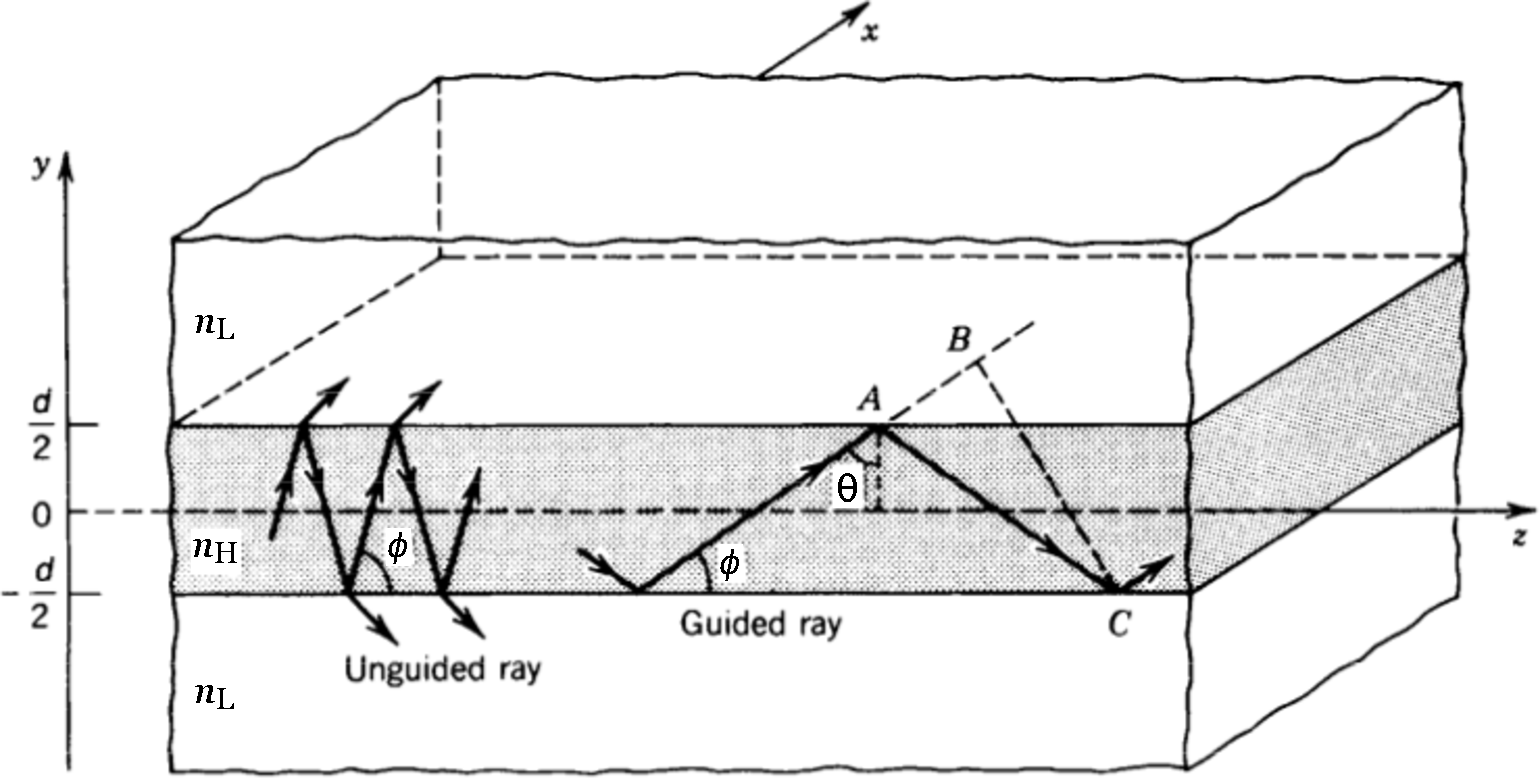
\includegraphics[scale=.4]{figures/dielBC.pdf}
	\tikzsetexternalprefix{tikz/}	% set subfolder
\tikzsetnextfilename{dielWG}
\begin{tikzpicture}
	\begin{axis}[	width=\textwidth*0.75,
								height=200pt,
								axis lines=center,
								xlabel={$z$}, ylabel={$y$},% zlabel={$y$},
								xmin=-0.1, xmax=+4.0,
								ymin=-1.6, ymax=+2.5,
								domain=0.5:3,
								xtick=\empty,
								ytick={-0.5,0.5},
								yticklabels={$-\dfrac{d}{2}$,$\dfrac{d}{2}$,},
								thick,
								area legend,
								legend style={draw=none},
								legend cell align=left,
								legend pos=outer north east,
								]

		\addplot [name path = top,] {+1.50};
		\addlegendentry{$n_L$}
		\addplot [name path = upper, 	forget plot] {+0.50};
		\addplot [name path = lower, 	forget plot] {-0.50};
		
		\addplot [pattern=crosshatch dots, pattern color=gray!50]
			fill between [ of=lower and upper];
		\addlegendentry{$n_H$}
		
		\draw [black] (0.5,-1.5) -- (3,-1.5);
		\draw [black] (0.5,-1.5) -- (0.5,+1.5);
		\draw [black] (3.0,-1.5) -- (3.0,+1.5);
		\draw [black] (3.0,-1.5) -- (3.8,-0.9) -- (3.8,+2.1) -- (3,+1.5);
		\draw [black] (0.5,+1.5) -- (1.3,+2.1) -- (3.8,+2.1);
		
		\path [name path= lowerFace, black] (3,-0.5) -- (3.8,+0.1);
		\path [name path= upperFace, black] (3,+0.5) -- (3.8,+1.1);
		\addplot [pattern=crosshatch dots, pattern color=gray!50]
			fill between [ of=lowerFace and upperFace];
		\draw [black] (3,-0.5) -- (3.8,+0.1) -- (3.8,+1.1) -- (3,+0.5);
		
		\draw [black, dashed] (1.3,+1.1) -- (3.8,+1.1);
		\draw [black, dashed] (1.3,+1.1) -- (1.3,+2.1);
		\draw [black, dashed] (1.3,+1.1) -- (0.5,+0.5);
		
		\draw [-stealth] (0,0) -- (0.4,0.3) node [above left] {$x$};
		
		\draw [	decoration={ markings, mark=between positions 0.0625 and 1 step 0.125 with {\arrow[line width=1]{stealth} }, }, postaction={decorate}]
			(0.8,-0.0) -- (0.88,+0.5) -- (1.06,-0.5) node [below] {\footnotesize Unguided ray} -- (1.22,+0.5) -- (1.38,-0.5) -- (1.46,+0.0);
			
		\draw [	decoration={ markings, mark=between positions 0.125 and 1 step 0.25 with {\arrow[line width=1]{stealth}}, }, postaction={decorate}]
			(1.7,-0.0) -- (2.0,+0.5) -- (2.6,-0.5) node [below left] {\footnotesize Guided ray} -- (2.9,+0.0);
		
		\draw [-stealth] (0.88,+0.5) -- (0.95, 0.65);
		\draw [-stealth] (1.22,+0.5) -- (1.29, 0.65);
		\draw [-stealth] (1.06,-0.5) -- (1.13,-0.65);
		\draw [-stealth] (1.38,-0.5) -- (1.45,-0.65);
		
	\end{axis}
\end{tikzpicture}
	\caption{Scheme of a dielectric slab waveguide, made by two materials with refractive indexes $n_H$ and $n_L$, with $n_H>n_L$.
		Two rays are shown: the unguided one is incident on the interface at an angle smaller than the critical angle.
		Conversely the guided ray is incident at a greater angle and is therefore totally reflected inside the waveguide \cite{Saleh1991}.}
	\label{fig:slabWG}
\end{figure}

2D-waveguides on the other hand are more common, to the point that with the term waveguide one usually refers to a device belonging to this category.
Since they confine light in two dimension, their core defines a path with which one can conduct light from a place to another.
A few types are shown in \autoref{fig:2DVG}.

\begin{figure}[ht]
	\centering
%	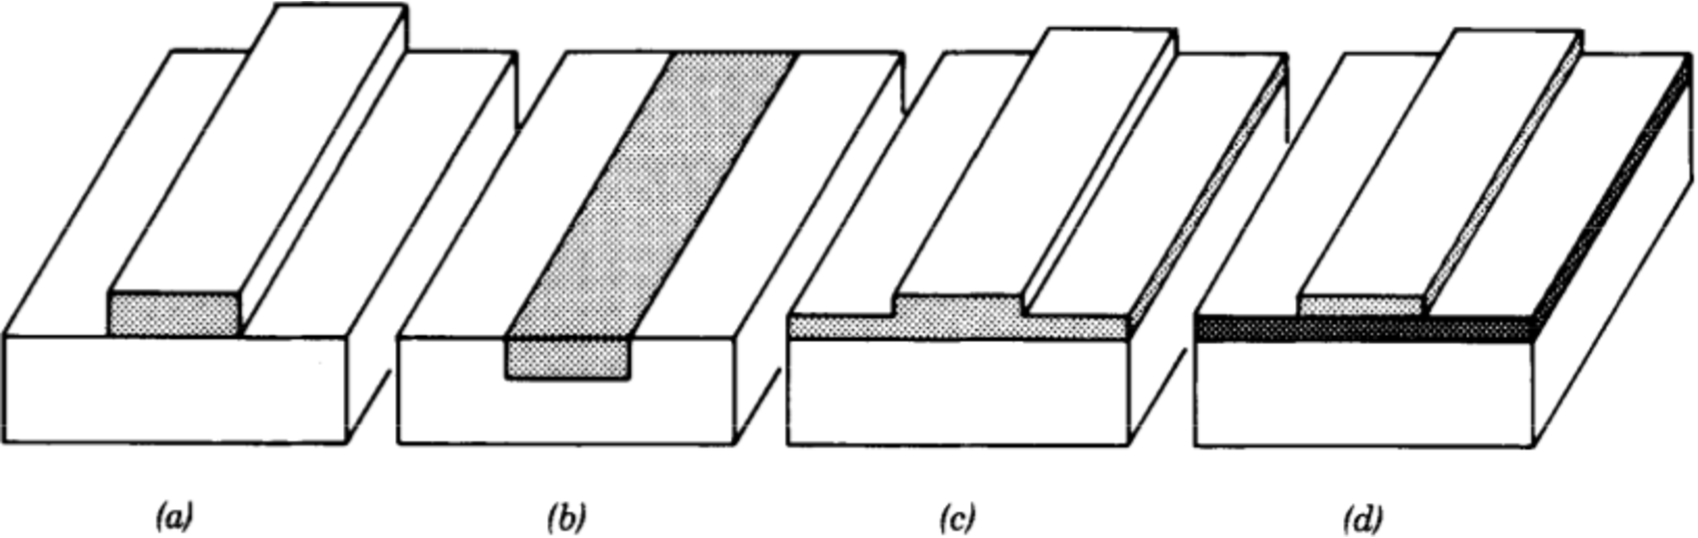
\includegraphics[scale=.4]{figures/WGtypes.pdf}
	\tikzsetexternalprefix{tikz/}	% set subfolder
\tikzsetnextfilename{WG_examples}
\begin{tikzpicture}[	scale=1,
										baseline,
										thick,
										line join=round,
										hatch/.style={
												preaction={fill, white},
												pattern=crosshatch dots,
												pattern color=gray
											},
										dense/.style={
												fill=gray!50,
%												preaction={fill, white},
%												pattern=crosshatch,
%												pattern color=black
											}
										]
%	\draw[step=.5,gray,very thin] (-.5,-.5) grid (12,3.5);

	\def\mylist{	0/0/2.4/0.75, 0.8/0.75/0.8/0.3,
							2.75/0/2.4/0.75,
							5.5/0/2.4/0.9, 6.3/0.9/0.8/0.15,
							8.25/0/2.4/0.9, 9.05/0.9/0.8/0.15
							}
	
	\foreach \px/\py/\w/\h in \mylist {
		\draw [fill=white]	(\px,\py) -- ++(0,\h) -- ++(60:2.4) -- ++(\w,0)
											-- ++(0,-\h) -- ++(240:2.4) -- cycle;
		\draw (\px,\py)++(\w,\h) -- ++(-\w,0)++(\w,0)
					-- ++(0,-\h)++(0,\h) -- +(60:2.4);
	}

	% first wg
	\draw [hatch] (0.8,0.75) -- ++(0,0.3) -- ++(0.8,0) -- ++(0,-0.3)	-- cycle;
	
	% second wg
	\draw [hatch] (2.75,0)++(0.8,0.75) -- ++(60:2.4) -- ++(0.8,0)
				-- ++(240:2.4) -- ++(0,-0.3) -- ++(-0.8,0) -- cycle;
	\draw (2.75,0)++(0.8,0.75) -- ++(0.8,0);	

	% third wg
	\draw [hatch] (5.5,0)++(0.8,0.9) -- ++(0,0.15) -- ++(0.8,0) -- ++(0,-0.15)
				-- ++(0.8,0) -- ++(0,-0.15) -- ++(-2.4,0) -- ++(0,0.15) -- cycle;
	\draw [hatch] (5.5,0)++(2.4,0.75) -- ++(0,0.15) -- ++(60:2.4) -- ++(0,-0.15) -- cycle;
	
	% fourth wg
	\draw [dense] (8.25,0)++(0,0.75) -- ++(0,0.15) -- ++(2.4,0) -- ++(60:2.4)
				-- ++(0,-0.15) -- ++(240:2.4) -- cycle;
	\draw (8.25,0)++(2.4,0.75) -- ++(0,0.15);
	\draw [hatch] (8.25,0)++(0.8,0.9) -- ++(0,0.15) -- ++(0.8,0) -- ++(0,-0.15) -- cycle;
	
	\foreach \px/\name in {1.2/a, 3.95/b, 6.7/c, 9.45/d}
		\node at (\px,0) [below] {$(\name)$};
\end{tikzpicture}
	\caption{Representation of a few types of 2D dielectric waveguides.
		Darker areas represent higher refractive index.
		Light is constrained in two direction and can only move forward or backward in the third direction.
		(a) strip, (b) embedded strip, (c) rib, (d) strip loaded \cite{Saleh1991}.
		}
	\label{fig:2DVG}
\end{figure}

Obviously, the versatility of straight (2D-) waveguides is limited.
Hence more complex structures such as bent waveguides have been developed.

\paragraph{Propagation of light inside waveguides\\}
\noindent A more complete description of guided modes is given by wave physics, where waveguides modes are described as superposition of planar transverse electro-magnetic (TEM) waves.
%Light propagates inside waveguides as superposition of transverse electro-magnetic (TEM) waves which keep reflecting on the interfaces of the core.
The result of the superposition is the so called \textit{mode}, which is expressed mathematically by
\begin{equation}
	\phi(\textbf{r}) = \phi_m\left( x, y \right) e^{i\left( \beta_m z - \omega t \right)}.
	\label{eq:mode_propagation}
\end{equation}
$\phi_m\left( x, y \right)$ is the transverse field distribution, $z$ is the direction of propagation, $\beta_m$ is the propagation constant of the m-th mode, and $\omega=2\pi \nu$ is the angular frequency of light.
Since light has two independent polarization, there are different modes for different polarizations.
Modes are therefore separated in \textit{transverse electric} (TE) and \textit{transverse magnetic} (TM), which propagates differently due to geometrical asymmetries.

Each mode, identified by the $m$ index, travels inside the waveguide with a certain propagation constant $\beta$ and maintaining a field distribution $\phi_m$.
Both of them depend on the materials and the geometry of the waveguide.
However, while $\beta_m$ decrease with increasing $m$ indexes, the features of the function $\phi_m$ grows in number.
Light often propagates in a manner described by a mode or superposition of them.
Usually other field distributions are rapidly scattered away.%, i.e. \textit{cannot propagate} inside the waveguide.

The field distribution of some of the first modes, in the simplest case of a slab waveguide, is represented in \autoref{fig:WGmodes}.
\begin{figure}[ht]
	\centering
%	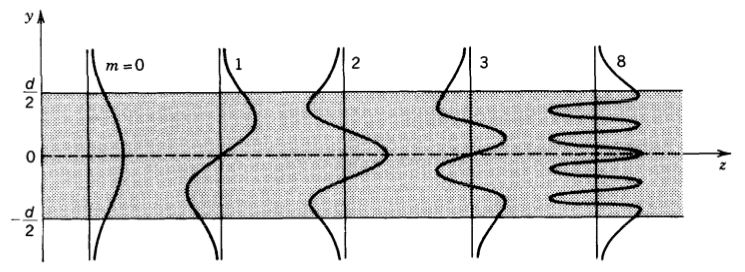
\includegraphics[scale=0.8]{figures/modes.png}
	\tikzsetexternalprefix{tikz/}	% set subfolder
\tikzsetnextfilename{WGmodes}
\begin{tikzpicture}[baseline]
	\begin{axis}[	width=\textwidth*0.75,
								height=200pt,
								axis lines=center,
								xlabel={$x$}, ylabel={$y$},
								xmin=-0.2, xmax=+4.0,
								ymin=-1.3, ymax=+1.3,
								domain=-1:1,
								xtick=\empty,
								ytick={-0.5,0.5},
								yticklabels={$-\dfrac{d}{2}$,$\dfrac{d}{2}$,},
								thick,
								area legend,
								legend style={draw=none},
								legend cell align=left,
								legend pos=outer north east,
								]
								
		\addlegendimage{black};
		\addlegendentry{$n_L$}
		\addplot [name path = upper, domain=0:3.8, 	forget plot] {+0.50};
		\addplot [name path = lower, domain=0:3.8,	forget plot] {-0.50};
		
		\addplot [pattern=crosshatch dots, pattern color=gray!50]
			fill between [ of=lower and upper];
		\addlegendentry{$n_H$}
		
		\addplot [black] ({0.5+.2    *exp(-8*x^2)}, {x});
		\addplot [black] ({1.0+.5*x  *exp(-8*x^2)}, {x});
		\addplot [black] ({1.5+2.*x^2*exp(-8*x^2)}, {x});
		\addplot [black] ({2.0+4.*x^3*exp(-8*x^2)}, {x});
%		
%		\draw [black] (0.5,-1.5) -- (3,-1.5);
%		\draw [black] (0.5,-1.5) -- (0.5,+1.5);
%		\draw [black] (3.0,-1.5) -- (3.0,+1.5);
%		\draw [black] (3.0,-1.5) -- (3.8,-0.9) -- (3.8,+2.1) -- (3,+1.5);
%		\draw [black] (0.5,+1.5) -- (1.3,+2.1) -- (3.8,+2.1);
%		
%		\path [name path= lowerFace, black] (3,-0.5) -- (3.8,+0.1);
%		\path [name path= upperFace, black] (3,+0.5) -- (3.8,+1.1);
%		\addplot [pattern=crosshatch dots, pattern color=gray!50]
%			fill between [ of=lowerFace and upperFace];
%		\draw [black] (3,-0.5) -- (3.8,+0.1) -- (3.8,+1.1) -- (3,+0.5);
%		
%		\draw [black, dashed] (1.3,+1.1) -- (3.8,+1.1);
%		\draw [black, dashed] (1.3,+1.1) -- (1.3,+2.1);
%		\draw [black, dashed] (1.3,+1.1) -- (0.5,+0.5);
%		
%		\draw [-stealth] (0,0) -- (0.4,0.3) node [above left] {$x$};
%		
%		\draw [	decoration={ markings, mark=between positions 0.0625 and 1 step 0.125 with {\arrow[line width=1]{stealth} }, }, postaction={decorate}]
%			(0.8,-0.0) -- (0.88,+0.5) -- (1.06,-0.5) node [below] {\footnotesize Unguided ray} -- (1.22,+0.5) -- (1.38,-0.5) -- (1.46,+0.0);
%			
%		\draw [	decoration={ markings, mark=between positions 0.125 and 1 step 0.25 with {\arrow[line width=1]{stealth}}, }, postaction={decorate}]
%			(1.7,-0.0) -- (2.0,+0.5) -- (2.6,-0.5) node [below left] {\footnotesize Guided ray} -- (2.9,+0.0);
				
	\end{axis}
\end{tikzpicture}
	\caption{Field distribution inside a slab waveguide.}
	\label{fig:WGmodes}
\end{figure}
The function inside the core is characterized by maxima, minima and nodes with a certain periodicity and the number of nodes is strictly linked to the index $m$.
Outside, the distribution of the field decays exponentially.
For waveguide with a 2D core, the field can be expected to be a multivariate version of similar functions.
However, differently from the analytical solution for slab waveguides, they are almost always found numerically.

The propagation constant can be written as
\begin{equation}
\beta_m = n_{eff} k_0 + i \alpha_{eff}/2
\end{equation}
where $k_0$ is the wavevector in vacuum, $n_{eff} \defeq c_0/v_{ph}$ is the \textit{effective refractive index}\index{effective refractive index} of the mode, and $\alpha_{eff}$ is \textit{effective absorption coefficient}\index{effective absorption coefficient}.
The effective refractive index is the ratio between the speed of light and the \textit{effective phase velocity} $v_{ph}$ at which each wavefront propagates in the core.
It is a pure number and its value is between the core refractive index and the cladding refractive index $n_L < n_{eff} < n_H$.
Given a WG geometry, larger $n_{eff}$ means a greater confinement of the electromagnetic field inside the core and a slower propagation speed along the waveguide.
The effective absorption coefficient instead is defined by the ratio between the input and output powers for a material of depth $L$, such that $I_{out}/I_{in}=e^{-\alpha_{eff}L}$, and has units of \si{\per\m}.
A low absorption coefficient is synonym of transparency and low power absorption per unit length.

%The physical interpretation of the effective indexes is that they define the propagation of the mode as a whole, instead of a superposition of multiple TEM waves each with a propagation characterized by the local values of refractive index and absorption coefficient.
%Moreover, in term of magnitudes, a higher refractive index means a slower propagation whereas a higher absorption coefficient means a higher power absorption per unit length.

%%The physical interpretation of the effective index is that of an average refractive index \textit{felt} by the mode propagating as a whole, instead of a superposition of multiple TEM waves \textit{feeling} different refractive indexes depending on the specific medium in which they are propagating.
%%Similarly, the effective absorption coefficient is linked to the ones of the materials, $n_{eff}$ is a complex number and the imaginary part is directly linked with the absorption properties of the materials.
%%Actually, a low imaginary part means that the material absorbs less and is therefore transparent to light.

Each one of these parameters, which describe the propagation of light along the waveguide, depends both on the materials and the geometry of the core and the cladding, but also on the frequency of light.
For dielectric waveguides, the fundamental mode ($m=0$) is always supported while higher modes might not be, depending both on the waveguides and on the frequency of light.
For this reason one distinguish \textit{single-mode} waveguides, which allow propagation for only the fundamental mode in a certain operative range of frequencies, from \textit{multi-mode} waveguides, which allow higher order modes to propagate.

Equation (\ref{eq:mode_propagation}) describes the propagation of a monochromatic light wave, which has ideally the same mode amplitude from $t=-\infty$ to $t=+\infty$.
This is obviously not a good physical representation, as light is generated and absorbed.
Eventually light is described to travel in wavepackets of finite duration, which are inherently non-monochromatic.

When light becomes non-monochromatic, the frequency dependence of the propagation constant $\beta$ has to be considered.
Usually, if working on a restricted range of frequencies, this dependence is characterized by a Taylor expansion at the second order.
\begin{subequations}
\begin{align}
	\beta\left(\omega\right)
		&\simeq \beta\left(\omega'\right)
						+ \frac{\partial \beta\left(\omega\right) }{\partial \omega} \Delta\omega
						+ \frac{1}{2}\frac{\partial^2 \beta\left(\omega\right) }{\partial \omega^2} \Delta\omega^2
				\label{eq:beta_taylor}\\
		&\simeq \dfrac{1}{v_{ph}} \omega'
						+ \frac{1}{v_g} \Delta\omega
						+ \frac{1}{2} \textsc{GVD}~ \Delta\omega^2
				\label{eq:beta_taylor_v}\\
		&\simeq \dfrac{n_{eff}}{c_0}\omega'
						+ \frac{n_{eff}^g}{c_0} \Delta\omega
						+ \frac{1}{2} \textsc{GVD}~ \Delta\omega^2
				\label{eq:beta_taylor_n}
\end{align}
\end{subequations}
where $\Delta\omega = \omega-\omega'$ and $\omega'$ is the frequency around which $\beta$ is expanded.
\autoref{eq:beta_taylor_v} is the same expansion, but the derivative are substituted by new quantities:
the \textit{phase velocity} $v_{ph}$, which describes the propagation speed of the wavefront of each frequency,
the \textit{group velocity} $v_g$, which describes the speed at which the ensemble of frequencies, the wavepacket, propagates, and finally the \textit{group velocity dispersion} $\textsc{GVD}$, which describes the relative behavior of the different frequency components in a single wavepacket.
Values of $\textsc{GVD} \neq 0 $ the wavepacket will either compress or dilate in time.
Those quantities are defined as follows:
%\begin{equation}
%v_{ph} \defeq \left( \dfrac{\beta}{\omega'}\right)^{-1}, \qquad
%v_{g}  \defeq \left( \dfrac{\partial \beta}{\partial \omega}\right)^{-1}, \qquad \mathrm{and} \qquad
%\textsc{GVD} \defeq \dfrac{\partial^2\beta}{\partial\omega^2} = \dfrac{\partial}{\partial\omega}\dfrac{1}{v_g}. 
%\end{equation}
\begin{subequations}
\begin{align}
v_{ph} &\defeq \left( \dfrac{\beta}{\omega'}\right)^{-1} \\
v_{g}  &\defeq \left( \dfrac{\partial \beta}{\partial \omega}\right)^{-1} \\
\textsc{GVD} &\defeq \dfrac{\partial^2\beta}{\partial\omega^2} = \dfrac{\partial}{\partial\omega}\dfrac{1}{v_g}.
\end{align}
\end{subequations}

On the other hand, it could be useful to express the propagation constant in terms of the effective refractive index, where $n_{eff} = c_0/v_{ph}$.
Then, similarly to the meaning of $n_{eff}$, one can define the \textit{effective group index} $n_{eff}^g$ as the ratio between the speed of light in vacuum $c_0$ and the effective group velocity $v_g$ of a packet of light inside a waveguide
\begin{equation}
	n_{eff}^g \defeq \dfrac{c_0}{v_g} = n_{eff}\left( \omega \right) +\omega\dfrac{\partial n_{eff}}{\partial \omega}
	\simeq n_{eff}\left( \lambda \right) -\lambda\dfrac{\partial n_{eff}}{\partial \lambda},
	\label{eq:neff_group}
\end{equation}
thus obtaining \autoref{eq:beta_taylor_n}.
%The latter equation allow to describe the Taylor expansion of $\beta$ in other terms:
%\begin{equation}
%	\beta\left(\omega\right) \simeq \frac{n_{eff}}{c_0}\omega' + \frac{n_{eff}^g}{c_0} \Delta\omega.
%	\label{eq:beta_taylor_n}
%\end{equation}

%To extend the description even further in the details of propagation, the Taylor expansion of \cref{eq:beta_taylor} can be truncated at the second order instead.
%This allow a more precise description of the wavepacket dynamics and introduces a new quantity, the \textit{group velocity dispersion}:
%\begin{equation}
%	GVD \defeq \dfrac{\partial^2\beta}{\partial\omega^2} = \dfrac{\partial}{\partial\omega}\dfrac{1}{v_g}.
%\end{equation}
%The \textsc{GVD}, defined as the second derivative of the propagation constant, is equivalent to the first derivative of the inverse of the group velocity.
%It describes the relative behavior of the different frequency components in a wavepacket.
%With a value of $\textsc{GVD} \neq 0 $ the wavepacket will either compress or dilate in time.

Nevertheless, our aim is to work in the quasi-static regime, i.e. to work with a time scale such that all measurable physical quantities converge to a finite value and do not show any time dependence.
Thus the monochromatic wave propagation description is still a valid model, because it is a very good approximation of slowly varying and almost monochromatic waves, such as the one I will use in my experiments.

\paragraph{Coupling of light between waveguides\\}
\label{par:light_coupling}
As shown in \autoref{fig:WGmodes}, the field distribution of modes propagating inside a slab waveguide is mainly contained inside the core.
However, the evanescent wave, i.e. the electromagnetic field outside the core, is non zero but decays exponentially from its value at the interface.
%The fact that the field outside is not zero but decays exponentially from its value at the interface allows to transfer optical power between waveguides that are sufficiently close.

%\textit{Evanescent coupling} exploits the fact that the evanescent field distribution outside the core decays exponentially to zero from its value at the interface \cite{Reed2008}.
\textit{Evanescent coupling} exploits the exponential decay of evanescent field outside the core to transfer light between two waveguides \cite{Reed2008}.
This means that when two waveguides are separated by a sufficiently small distance, the field distribution of one waveguide cannot decay sufficiently fast and instead extends itself over the core of the second waveguide.
When this happens, optical power is transferred between the waveguides.

The simpler case is obtained when two parallel straight waveguides are separated by a small distance, a gap, and the field is non zero only at the input of one of them.
Therefore light propagates along the waveguide, its evanescent field overlaps with the core of the second waveguide.
Light is then \textit{coupled} inside the second waveguide as it propagates along the first waveguide and power is transferred between the waveguides.

The maximum value of power transferred per unit length is determined mainly by the distance between the waveguides.
The larger the gap, the lower will be the its value.
Moreover, the exchange of optical power is a periodic function of the propagating distance.
%Hence, the length of the coupling region is the second most important parameter that determines the portion of optical power exchanged in the end.
Depending on the specific materials and on the geometry of the coupling region, a known amount of light can be coupled between the waveguides.

\newpage
\subsection{Microring optical cavity}
\label{ssec:Microring_optical_cavity}
In integrated photonics the microring is an optical cavity made by bending a waveguide on itself.
To insert light into the cavity, the microring is often side coupled with one or two straight waveguides.
Light inserted from the different ports into the cavity interfere with itself, after a round trip.
When the waves are in phase, they generate constructive interference and the energy stored in the cavity increases exponentially.
On the other hand, when the signals are out of phase, the interference is destructive and no energy is stored in the cavity.

\begin{figure}[ht]
	\centering
%	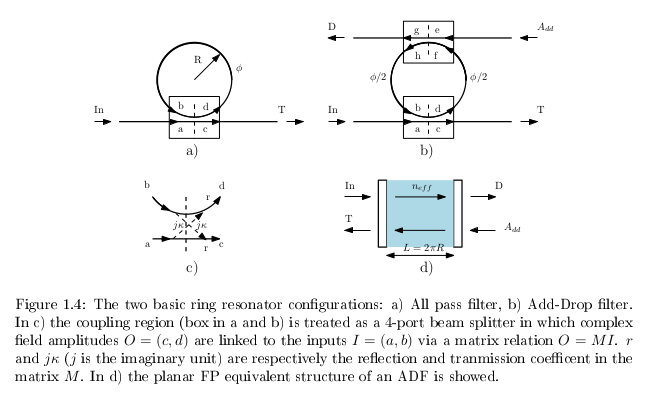
\includegraphics[scale=.8]{figures/microring_theory.png}
	\begin{subfigure}[b]{0.3\textwidth}
		\centering
		\tikzsetexternalprefix{tikz/}	% set subfolder
\tikzsetnextfilename{APF_scheme}
\begin{tikzpicture}[baseline, thick, every node/.style={font=\scriptsize}]
	\draw [{stealth[reversed]}-stealth] (-1.5,0)
				node [below] {input} -- (1.5,0)
				node [below] {through};
	\draw [{stealth[reversed]}-stealth] (-0.5,0) -- (0.5,0);
	
	\draw (0,1) circle (0.9);
	\draw [-{stealth}] (0,1)
				-- ++(30:0.9cm) node [midway, below right] {R};
	
	\draw [-{stealth}] (0,0.1)
				arc [start angle=-90,end angle=-60, radius=0.9];
	\draw [-{stealth[reversed]}] (0,0.1)
				arc [start angle=-90,end angle=-120, radius=0.9];
	
	\draw [thin, densely dashed] (0,-0.2) -- (0,0.3);	
	
	\draw [thin]		(-0.5,0.4) -- (+0.5,0.4) --
								(+0.5,-0.3) -- (-0.5,-0.3) -- cycle;
\end{tikzpicture}
		\caption{APF}
		\label{fig:APF_scheme}
	\end{subfigure}
	\hspace{.02\textwidth}
	\begin{subfigure}[b]{0.3\textwidth}
		\centering
		\tikzsetexternalprefix{tikz/}	% set subfolder
\tikzsetnextfilename{ADF_scheme}
\begin{tikzpicture}[baseline, thick, every node/.style={font=\scriptsize}]
	% lowe line & arrows
	\draw [{stealth[reversed]}-stealth] (-0.5,0) -- (+0.5,0);
	% lower long line
	\draw [{stealth[reversed]}-stealth] (-1.5,0)
				node [below] {input} -- (1.5,0)
				node [below] {through};
	% lower ring
	\draw [-{stealth}] (0,0.1)
				arc [start angle=-90,end angle=-60, radius=0.9];
	\draw [-{stealth[reversed]}] (0,0.1)
				arc [start angle=-90,end angle=-120, radius=0.9];
	% lower box
	\draw [thin, densely dashed] (0,-0.2) -- (0,0.3);	
	\draw [thin]		(-0.5,0.4) -- (+0.5,0.4) --
								(+0.5,-0.3) -- (-0.5,-0.3) -- cycle;

	% circle
	\draw (0,1) circle (0.9);
	% radius arrow
	\draw [-{stealth}] (0,1)
				-- ++(30:0.9cm) node [midway, below right] {R};

	% upper lines & arrows
	\draw [{stealth[reversed]}-stealth] (+0.5,2) -- (-0.5,2);
	% upper long line
	\draw [{stealth[reversed]}-stealth] (+1.5,2)
				node [above] {add} -- (-1.5,2)
				node [above] {drop};
	% upper ring
	\draw [-{stealth[reversed]}] (0,1.9)
				arc [start angle=+90,end angle=+60, radius=0.9];
	\draw [-{stealth}] (0,1.9)
				arc [start angle=+90,end angle=+120, radius=0.9];
	% upper box
	\draw [thin, densely dashed] (0,2.2) -- (0,1.7);	
	\draw [thin]		(-0.5,1.6) -- (+0.5,1.6) --
								(+0.5,2.3) -- (-0.5,2.3) -- cycle;
\end{tikzpicture}
		\caption{ADF}
		\label{fig:ADF_scheme}
	\end{subfigure}
	\hspace{.02\textwidth}
	\begin{subfigure}[b]{0.3\textwidth}
		\centering
		\tikzsetexternalprefix{tikz/}	% set subfolder
\tikzsetnextfilename{APF-ADF_coupling_scheme}
\begin{tikzpicture}[baseline, line width=8pt, every node/.style={font=\small}]
	\draw [gray!30] (0,0) node [above, black] {$E^{r-}$}
				arc [start angle=-105,end angle=-75, radius=5] node [above, black] {$E^{r+}$};
	\draw [gray!30] (0,-0.8) node [below, black] {$E^{w-}$}
				-- (2.588190451,-0.8) node [below, black] {$E^{w+}$};

	\draw [thin, densely dashed] (1.294095225,-1.5) -- (1.294095225,.5);

	\draw [thin, dashed, {stealth[reversed]}-stealth, out=-15, in=180] (0,0)
				to node [pos=0.4, left]	{$i\kappa$} (2.588190451,-0.8);
	\draw [thin, dashed, {stealth[reversed]}-stealth, out=0, in=195] (0,-0.8)
				to node [pos=0.6, right]	{$i\kappa$} (2.588190451,-0.0);

	\draw [thin, dashed, {stealth[reversed]}-stealth] (0,0)
				arc [start angle=-105,end angle=-75, radius=5]
				node [midway, above right] {$\tau$};
	\draw [thin, dashed, {stealth[reversed]}-stealth] (0,-0.8)
				-- (2.588190451,-0.8) node [midway, below right] {$\tau$};
\end{tikzpicture}
		\caption{Coupling region}
		\label{fig:coupling_scheme}
	\end{subfigure}
	
	\caption{
		Schematic representation of microring configurations and of their coupling regions.
		APF has two channels, \textit{input} and \textit{through}, and one coupling region.
		ADF has four channels, \textit{input}, \textit{through}, \textit{add} and \textit{drop}, and two coupling regions.
		The coupling constants ($\kappa$ and $\tau$) are in principle different for each coupling region.
	}
	\label{fig:resonator_theory}
\end{figure}

In the simpler case when there is only one waveguide side coupled to the resonator the optical cavity has only two ports, which are usually called \textit{input} and \textit{through}.
This configuration, shown in \autoref{fig:APF_scheme}, is called \textit{All-Pass Filter}, because in the ideal case, where no losses happen, all the signal passes from the input to the through channels.
%All pass resonators have only one input and one output: light then propagate in only in one direction, unless some specific phenomena happens (e.g. back scattering).

By adding a secondary waveguide coupled to the ring, one obtains the so called Add-Drop Filter (ADF) configuration, shown in \autoref{fig:ADF_scheme}.
Its name derives from the fact that the two additional ports are called \textit{add} and \textit{drop} respectively.
This simple structure can be readily used as a signal mixer: signals at the resonance wavelengths of the cavity are directed from the input to the drop channel or from the add channel to the through port.
Additionally signals out of resonance travel straight from the input to the through channel and from the add to the drop port.
%Resonators with more than four ports are possible, however are very uncommon.

In both configurations light is transferred from the waveguides to the microring within the \textit{coupling regions}, as shown in \autoref{fig:coupling_scheme}.
The simplest model considers the region as infinitely small compared to the other dimensions.
However the model can be expanded to include coupling regions with a finite length, which transform the microring in the so called \textit{racetrack resonator}.

The theoretical model usually employed to describe resonators analytically decomposes their structure in a series of simpler substructures.
Both the APF and the ADF configurations are studied as ordered combinations of straight waveguides, coupling regions, and bent waveguides.
Other used descriptions, such as numerical simulation obtained with finite element methods (FEM), achieve more precise results, however they are more dependent on the specific geometry of the problem.
Moreover the approximation given by the analytical model is sufficiently accurate to make quantitative prediction of the coupling and it gives a clear description of the physics behind it.
Furthermore it can be expanded to include non-trivial phenomena (see \autoref{sec:Nonlinear_Optics}).
In the following section I will go through the necessary steps to solve the case of the ADF configuration in the theoretical model.

%1.2.3.2 Add-drop filter theory\\
\subsubsection{Add-Drop-Filter theory}
\label{sssec:Add-Drop-Filter_theory}
ADF configuration is obtained when a microring is coupled to two waveguides.
Such structure is composed by three different basic structures: four straight waveguides, two bent waveguides which together form the whole ring, and two coupling regions between the waveguides and the microring.
Each of these pieces transfers light to or from the outside or another piece.

Since our experiments are carried out in a time scale such that physics phenomena can be considered quasi-static, the field propagating in the device is described by a scalar complex function which, assuming a monochromatic continuous EM wave, loses any temporal dependence:
\begin{equation}
	E(z) = |E(z_0)|e^{i\beta z},
\end{equation}
where $z$ is the direction of propagation, loosely defined to accommodate propagation both along straight and bent waveguides ($z\sim r\theta$), $t$ is time, $\omega=2\pi\nu$ is the angular frequency, and $\beta = n_{eff}k_0+i\alpha_{eff}/2$ is the propagation constant.
Both dependence of the effective index $n_{eff}=n_{eff}\left(\omega\right)$ and the effective loss factor $\alpha_{eff}=\alpha_{eff}\left(\omega\right)$ will be expanded only when necessary.

Generally the propagation along the straight waveguides is considered lossless (i.e. $\alpha_{eff}\approx 0$), while the propagation along the two bent regions has a non negligible loss (i.e $\alpha_{eff}> 0$).
%Propagation in the straight waveguides is often considered without loss (i.e. $\alpha_{eff}\approx 0$) and thus neglected.
%On the other hand, propagation in the two halves of the ring is frequently considered with radiative losses (i.e $\alpha_{eff}> 0$), because a bent waveguide is intrinsically more difficult to fabricate in comparison to a straight one.
The coupler between the resonator and the waveguides is considered like a beamsplitter.
In this approximation, light does not propagate in this part as it was in the previous ones.
Its operation is reduced to the exchange of power between the two input ports and two output ports, which is described by the following matrices:
\begin{equation}
\begin{pmatrix}
E^{w+}_{ch} \\
E^{r+}_{ch} \\
\end{pmatrix} = \textbf{M}
\begin{pmatrix}
E^{w-}_{ch} \\
E^{r-}_{ch} \\
\end{pmatrix}, \qquad \textbf{M} = 
\begin{pmatrix}
\tau & i\kappa \\
i\kappa & \tau \\
\end{pmatrix},
\end{equation}
where $E$ is the field amplitude of the `$_{ch}$' channel either in the waveguide `$^w$' or in the ring `$^r$', before `$^-$' and after `$^+$' the coupling.
An explanatory diagram is shown in \autoref{fig:coupling_scheme}.
The matrix $\textbf{M}$ is characterized by two real valued parameters, $\tau$ and $\kappa$, between $0$ and $1$.
Specifically, they must verify the following constraint:
\begin{equation}
\det\left(\textbf{M}\right) = |\tau|^2 + |i\kappa|^2 = 1.
\end{equation}
which represents the conservation of energy.

At this point one can solve the problem by putting all the pieces together.
Neglecting the propagation inside the waveguide, the full system of equation that describe the problem is:
\begin{subequations}
\begin{align}
E^{w+}_{in}	&= \tau 		 E^{w-}_{in} + i\kappa	E^{r-}_{in} \label{seq:in_w+}\\
E^{r+}_{in}	&= i\kappa	 E^{w-}_{in} + \tau 		E^{r-}_{in} \label{seq:in_r+}\\
\nonumber\\
E^{r-}_{out}	&= E^{r+}_{in}		e^{i\beta \pi R } \label{seq:out_r-_in}\\
E^{r-}_{in}	&= E^{r+}_{out}	e^{i\beta \pi R } \label{seq:in_r-_out}\\
\nonumber\\
E^{w+}_{out}	&= \tau 		 E^{w-}_{out} + i\kappa	E^{r-}_{out} \label{seq:out_w+}\\
E^{r+}_{out}	&= i\kappa	 E^{w-}_{out} + \tau 		E^{r-}_{out} \label{seq:out_r+}
\end{align}
\label{eq:ADF_equations}
\end{subequations}
The first two \cref{seq:in_w+,seq:in_r+} describe the exchange of optical power between the first channel and the microring resonator (see $in$ box in \autoref{fig:ADF_scheme}).
Then the third and fourth \cref{seq:out_r-_in,seq:in_r-_out} delineate the propagation of light in the two halves of the resonator, from one coupling region to the other.
Lastly the remaining two equation characterize the transfer of light between the resonator and the add-drop channel (see $out$ box in \autoref{fig:ADF_scheme}).

Using these equations it is easy to define new quantities of interest: the first one is the transmittance from the \textit{input} to the \textit{through} port.
\begin{equation}
\eta_T\left(\omega\right) \defeq \dfrac{E^{w+}_{in}}{E^{w-}_{in}}
	= t\dfrac{1-e^{i\beta 2\pi R}}{1-\tau^2e^{i\beta 2\pi R}}
\end{equation}
Similarly, one can also define the transmittance from the \textit{input} to the \textit{drop} port.
\begin{equation}
\eta_D\left(\omega\right) \defeq \dfrac{E^{w+}_{out}}{E^{w-}_{in}}
	= \dfrac{-\kappa^2e^{i\beta\pi R}}{1-\tau^2e^{i\beta 2\pi R}}
\end{equation}

However, this quantities have complex values and therefore are difficult to study.
For this reason, one usually defines the transmission between the same ports as the square modulus of the transmittance.
Thus it follows that
\begin{equation}
T \left( \omega \right) \defeq |\eta_T|^2 = \tau 
\dfrac	{ \left( 1- 				\gamma \right)^2 + 4 				\gamma \sin^2 \left( n_{eff} k_0 \pi R \right) }
			{ \left( 1-\tau^2	\gamma \right)^2 + 4 \tau^2	\gamma \sin^2 \left( n_{eff} k_0 \pi R \right) }
\end{equation}
and
\begin{equation}
D \left( \omega \right) \defeq |\eta_D|^2 =
\dfrac	{ \kappa^4 \gamma}
			{ \left( 1-\tau^2	\gamma \right)^2 + 4 \tau^2	\gamma \sin^2 \left( n_{eff} k_0 \pi R \right) }
\end{equation}
where the notation is simplified by loss parameter $\gamma = e^{-\alpha_{eff}\pi R}$.
The dependence of $T=T(\omega)$ and $D=D(\omega)$ from the frequency (or wavelength) of light is obtained by making explicit the wavevector dependence $k_0=\frac{\omega}{c_0}=\frac{2\pi}{\lambda}$ in which $c_0$ is the speed of light in vacuum.

Apart from a simpler description, transmission is directly connected with the optical power as it represent the ratio between the input and output power.
%The transmission is much more easy to study than the transmittance because it is real valued.
%Moreover it is physically significant as it represents the ratio between the input and output optical powers.
In fact, the optical power is defined as the square modulus of the optical field, except for a constant factor:
$$ I = \frac{1}{2}n_0c_0|E|^2 \propto |E|^2$$
Both transmission spectra, as shown in \autoref{fig:ADF}, have either peaks or dips: at each microring resonance, the through spectrum shows dips while the drop spectrum shows peaks.
The depth of the dips, the height of the peaks, and the width of both of them is defined by few parameters: the coupling constant $\tau$\footnote{one can choose also $\kappa$, but it does not matter which one, since $\tau^2 = 1-\kappa^2$} and the half round trip loss factor $\gamma = e^{-\alpha_{eff}\pi R}$.

\begin{figure}[htbp]
	\centering
	\tikzsetexternalprefix{tikz/}	% set subfolder
\tikzsetnextfilename{ADF}
\begin{tikzpicture}
	\newcommand\CENTRAL{193}
	\newcommand\START{193-5}
	\newcommand\STOP {193+7}
	\newcommand\CC{299792458}
	
	\begin{axis}[%
			axis x line*= bottom,
%			scaled x ticks = manual:{$+\SI{193}{\THz}$}{ \pgfmathparse{#1-\CENTRAL} },%
			xlabel = {Optical Frequency $\nu$ [$\si{\THz}$]},
			ylabel = {Transmission},
			legend columns=3,
			legend cell align=right,
			legend style={ at={(0.5,-0.22)}, anchor=north },
			width=\textwidth*0.75,%
			height=207pt,
			xmin= 188, xmax = 199,
			%
			% global plot definition
			domain = \START:\STOP,
			samples = 551,
			smooth,
			no markers,
			cycle multi list={
%					exotic\nextlist 
					color list\nextlist
					solid,densely dotted
					%[2 of]linestyles
				},
			]
				
		\foreach \TA/\LA/\Radius/\Neff in {0.85/0.9/5/3.826, 0.85/0.75/5/3.826 }{ %, 0.9/0.99/5/3.826
			\edef\temp{
				\noexpand\addlegendimage{empty legend}
				\noexpand\addlegendentry{$\tau=\TA,\gamma=\LA,R=\SI{\Radius}{\um}:$};
				\noexpand\addplot 
										{ + (1-\TA^2)^2 * \LA
											/ ( (1-\TA^2 * \LA)^2 	+ 4 * \TA^2 	* \LA *sin(deg(\Neff*pi*\Radius*2*pi*x*1e6/\CC))^2 )
										};
				\noexpand\addlegendentry{$D(\omega)$};
				\noexpand\addplot 
										{ + \TA^2 * ( (1- \LA)^2	+ 4 					* \LA *sin(deg(\Neff*pi*\Radius*2*pi*x*1e6/\CC))^2 )
											/ ( (1-\TA^2 * \LA)^2 	+ 4 * \TA^2 	* \LA *sin(deg(\Neff*pi*\Radius*2*pi*x*1e6/\CC))^2 )
										};
				\noexpand\addlegendentry{$T(\omega)$};
								}
			\temp
		}
		
		\draw [|<->|] (192.0446013229, 0.6) -- (194.5386870543, 0.6) node [midway, fill=white] {$FSR$};%0.5665693
	
		\draw [<-] (192.3, 0.283) -- (193.1,0.283) node [right] {$\Delta\omega$}; %0.5665693/2 = 0.283
		\draw [<-] (191.8, 0.283) -- (191,0.283) {};	
		
	\end{axis}
	
	\begin{axis}[
			width=\textwidth*0.75,%
			height=207pt,
			axis x line*= top,
			axis y line = none,
			xlabel = {Wavelength $\lambda$ [\si{\nm}]},
			xmin= 188, xmax = 199,
%			xmin= 150, xmax = 250,
%  		xtick = {187.37029,188.54872,189.74206,190.95061,192.17465,193.41449,194.67043,195.94278,197.23188,198.53805,199.86163},
			xtick = {187.37029,188.54872,189.74206,190.95061,192.17465,193.4143 ,194.67043,195.94278,197.2318 ,198.53805,199.86163},
%			xtick = {157.785504211, 171.309976, 187.37029, 199.86163, 214.13747, 230.609583077, 249.827048333},
%			scaled x ticks = manual:{$+\SI{1500}{\nm}$}{ \pgfkeys{/pgf/fpu}\pgfmathparse{(1e-3*\CC/#1) - 1500} },
			scaled x ticks = manual:{}{ \pgfkeys{/pgf/fpu}\pgfmathparse{(1e-3*\CC/#1)} },
		]
		\addplot[black, opacity=0, domain = \START:\STOP] {0}; %
	\end{axis}
\end{tikzpicture}
	\caption{
		Transmission spectra of microring resonators in ADF configuration for the through $T(\omega)$ and drop ports $D(\omega)$.
		The resonators considered differ in radius ($R=$\SI{4}{\um} and $R=$\SI{5}{\um}), but share the coupling constant $\tau=0.85$, the half round trip loss factor $\gamma=0.8$ and the effective index $n_{eff}=3.826$.
	}
	\label{fig:ADF}
\end{figure}

The frequency of each resonance is identified by a positive integer number, that verifies the following equation:
\begin{equation}
	\omega_m = m\dfrac{c_0}{n_{eff}(\omega)R},
\end{equation}
where the dependence of $n_{eff}=n_{eff}\left(\omega\right)$ has been explicitly shown.

Each resonance is spaced from the next one by a quantity called \textit{Free Spectral Range}\index{Free Spectral Range (FSR)} $FSR_{\omega_m}$.
By exploiting the Taylor expansion of $\beta$ seen in \cref{eq:beta_taylor_n} one obtains
\begin{equation}
	FSR_{\omega_m} \simeq \dfrac{c_0}{n_{eff}^g\left(\omega_m\right) R} .
\end{equation}
where the \textit{effective group index} $n_{eff}^g\left(\omega\right)$ has been defined in \cref{eq:neff_group}.
Another important quantity is the width of the peaks or dips of each resonance.
Ordinarily one evaluates the so called \textit{full-width-half-maximum} (FWHM) of the transmission in the drop channel:
\begin{equation}
	FWHM_{\omega_m} = \dfrac{c_0}{n_{eff}^g\left(\omega_m\right)}\dfrac{1- \tau^2\gamma}{\pi R \tau \sqrt{\gamma}}
\end{equation}
\autoref{fig:ADF2} shows both the $FSR$ and the $FWHM$ for a family of resonances.

\begin{figure}[htbp]
	\centering
	\tikzsetexternalprefix{tikz/}	% set subfolder
\tikzsetnextfilename{ADF2}
\begin{tikzpicture}[baseline]
	\newcommand\CENTRAL{193}
	\newcommand\START{193-5}
	\newcommand\STOP {193+7}
	\newcommand\CC{299792458}
	
	\begin{axis}[%
			axis x line*= bottom,
%			scaled x ticks = manual:{$+\SI{193}{\THz}$}{ \pgfmathparse{#1-\CENTRAL} },%
			xlabel = {Optical Frequency $\nu$ [$\si{\THz}$]},
			ylabel = {Transmission},
			legend columns=3,
			legend cell align=right,
			legend style={ at={(0.5,-0.22)}, anchor=north },
			/pgf/number format/1000 sep=,
			width=\textwidth*0.75,%
			height=207pt,
			xmin= 188, xmax = 199,
			%
			% global plot definition
			domain = \START:\STOP,
			samples = 551,
			smooth,
			no markers,
			cycle multi list={
%					exotic\nextlist 
					color list\nextlist
					solid,densely dotted
					%[2 of]linestyles
				},
			]
				
		\foreach \TA/\LA/\Radius/\Neff in {0.85/0.9/5/3.826, 0.85/0.75/5/3.826 }{ %, 0.9/0.99/5/3.826
			\edef\temp{
				\noexpand\addlegendimage{empty legend}
				\noexpand\addlegendentry{$\tau=\TA,\gamma=\LA,n_{eff}=\Neff, R=\SI{\Radius}{\um}:$};
				\noexpand\addplot 
										{ + (1-\TA^2)^2 * \LA
											/ ( (1-\TA^2 * \LA)^2 	+ 4 * \TA^2 	* \LA *sin(deg(\Neff*pi*\Radius*2*pi*x*1e6/\CC))^2 )
										};
				\noexpand\addlegendentry{$D(\omega)$};
				\noexpand\addplot 
										{ + \TA^2 * ( (1- \LA)^2	+ 4 					* \LA *sin(deg(\Neff*pi*\Radius*2*pi*x*1e6/\CC))^2 )
											/ ( (1-\TA^2 * \LA)^2 	+ 4 * \TA^2 	* \LA *sin(deg(\Neff*pi*\Radius*2*pi*x*1e6/\CC))^2 )
										};
				\noexpand\addlegendentry{$T(\omega)$};
								}
			\temp
		}
		
		\draw [|<->|] (192.0446013229, 0.6) -- (194.5386870543, 0.6) node [midway, fill=white] {\scriptsize $FSR$};%0.5665693
	
		\draw [<-] (192.3, 0.283) -- (192.8,0.283) node [right] {\scriptsize $FWHM$}; %0.5665693/2 = 0.283
		\draw [<-] (191.8, 0.283) -- (191.3,0.283) {};
		
	\end{axis}
	
	\begin{axis}[
			width=\textwidth*0.75,%
			height=207pt,
			axis x line*= top,
			axis y line = none,
			xlabel = {Wavelength $\lambda$ [\si{\nm}]},
			xmin= 188, xmax = 199,
%			xmin= 150, xmax = 250,
%  		xtick = {187.37029,188.54872,189.74206,190.95061,192.17465,193.41449,194.67043,195.94278,197.23188,198.53805,199.86163},
			xtick = {187.37029,188.54872,189.74206,190.95061,192.17465,193.4143 ,194.67043,195.94278,197.2318 ,198.53805,199.86163},
%			xtick = {157.785504211, 171.309976, 187.37029, 199.86163, 214.13747, 230.609583077, 249.827048333},
%			scaled x ticks = manual:{$+\SI{1500}{\nm}$}{ \pgfkeys{/pgf/fpu}\pgfmathparse{(1e-3*\CC/#1) - 1500} },
			scaled x ticks = manual:{}{ \pgfkeys{/pgf/fpu}\pgfmathparse{(1e-3*\CC/#1)} },
			/pgf/number format/1000 sep=,
		]
		\addplot[black, opacity=0, domain = \START:\STOP] {0}; %
	\end{axis}
\end{tikzpicture}
	\caption{
		Transmission spectra of microring resonators in ADF configuration for the through $T(\omega)$ and drop ports $D(\omega)$.
		The microring has radius $R=\SI{5}{\um}$ and effective index $n_{eff}=3.826$.
		The coupling constant is $\tau=0.85$, while the loss factor $\gamma$ takes two values: $0.9$ (red) and $0.75$ (blue).
		The arrows indicate a $FSR_\nu \approx \SI{2.49}{\THz}$ and a $FWHM_\nu \approx \SI{0.35}{\THz}$, which gives a quality factor of around $Q \approx \num{550}$.
		The blue curve has $FWHM_\nu \approx \SI{0.5}{\THz}$ and $Q \approx \num{390}$.
		Each resonance is identified by its positive integer number.
	}
	\label{fig:ADF2}
\end{figure}

Values such this are often expressed in the wavelength domain:
\begin{equation}
	FSR_{\lambda_m} \simeq \dfrac{\lambda_m^2}{n_{eff}^g\left(\lambda_m\right) 2\pi R}
		\qquad \mathrm{and} \qquad
	FWHM_{\lambda_m} \simeq	\dfrac{\lambda_m^2}{n_{eff}^g}
													\dfrac{1- \tau^2\gamma}{2\pi^2 R \tau \sqrt{\gamma}}
\end{equation}
where $n_{eff}^g\left(\lambda_m\right)$ is the appropriate redefinition of the effective group index in the wavelength domain, shown in \cref{eq:neff_group}.

Another important quantity to describe an optical resonator response is the \textit{enhancement factor} $EF$.
It is defined as the ratio between the incident optical power $I_{inc}$ and the power circulating inside the cavity $I_{ins}$:
\begin{equation}
EF
	\defeq \dfrac{I_{int}}{I_{inc}}
	\simeq \dfrac{|E_{in}^{r+}|^2}{|E_{in}^{w-}|^2}
	= \dfrac	{ \kappa^2 } { \left( 1-\tau^2	\gamma \right)^2 + 4 \tau^2	\gamma \sin^2 \left( n_{eff} k_0 \pi R \right) },
	\label{eq:enhancement_factor}
\end{equation}
where in the last equality, I assumed low loss waveguides $\gamma \rightarrow 1$.
This assumption allows to consider the field at an arbitrary position along the ring.

Finally, an additional figure of merit is the important quantity is the \textit{quality factor} $Q-factor$, or simply $Q$.
It has many similar definitions, depending on the field of study.
The most physical, but less operative one defines $Q$ as $2\pi$ times the ratio between the energy stored in the cavity and the energy lost each cycle.
\begin{equation}
	Q \defeq 2\pi \times \frac{\mathrm{energy~stored}}{\mathrm{energy~lost~per~cycle}}
\end{equation}
However, for my purposes this definition is too cumbersome, thus I used a similar one instead:
\begin{equation}
	Q \defeq \dfrac{\omega_m}{FWHM_{\omega_m}} = \dfrac{\lambda_m}{FWHM_{\lambda_m}}
\end{equation}
Both are sensible definitions and as $Q$ becomes larger they become approximately equivalent.

Physically, the quality factor is linked to the photon lifetime in cavity $t_m$ by the relation
\begin{equation}
	Q \simeq \frac{\omega_m}{FWHM_{\omega_m}} \propto \omega_m t_m.
\end{equation}
From this description one can observe that higher quality factors mean longer photon lifetimes.
This is due to the fact that the photon lifetime is strictly dependent on the losses of the cavity and the $Q$ factor is inversely related to them.
However, in an optical cavity losses are given by absorption, but also by the coupling of the input and output channels.
Thus, given a certain waveguide loss (defined by both the propagation and radiative contributions), the same Q-value can be obtained by different sets of loss factors.
One can identify three distinct regimes: over-coupling, critical-coupling, and under-coupling regimes.
\autoref{fig:Q_contour} shows contour plots of the maximum transmission in the drop channel and the quality factor as functions of the cavity losses ($\gamma$) and the coupling coefficients ($\kappa^2=1-\tau^2$).

\begin{figure}[!hbtp]
	\centering
	\begin{subfigure}[t]{0.5\textwidth}
		\centering
%		\tikzsetexternalprefix{tikz/}	% set subfolder
\tikzsetnextfilename{ADF_D_contour}
\begin{tikzpicture}[baseline]
	
	\begin{axis}[
			title = {$D\left( \omega_{m} \right)$},
			width=8cm, % height=207pt,
			domain = 0:1,
			xmax=1,
			xlabel = {$\tau^2$},
			ylabel = {$\gamma$},
			samples = 101,
			view={0}{90},
			]
		
		\addplot3 [contour gnuplot={
								labels over line,
								levels={0.01,0.05,0.1,0.25,0.5,0.75,0.9},
								handler/.style=smooth,
								label distance=150pt,
								contour label style={
										/pgf/number format/fixed,
										/pgf/number format/precision=2,
									},
								}
		] {(1-x)^2*y/(1-x*y)^2	};
	\end{axis}
	
\end{tikzpicture}
		\tikzsetexternalprefix{tikz/}	% set subfolder
\tikzsetnextfilename{ADF_D_logx_contour}
\begin{tikzpicture}[baseline]
	
%% logx contour plot	
	\begin{axis}[
			title = {$D\left( \nu_{m} \right)$},
			width=8cm, % height=207pt,
			domain = -2:0,
			domain y = 0:1,
			xmin=-2, xmax=0,
			ymin=+0, ymax=1,
			xtick=\empty,
			ylabel = {$\gamma$},
			yticklabel pos=right,
			samples = 51,
			view={0}{90},
			colormap/bluered,
			thick,
			]
		
		\addplot3 [contour gnuplot={
								labels over line,
								levels={0.01,0.05,0.1,0.25,0.5,0.75},%,0.9},
								label distance=200pt,
								contour label style={
										/pgf/number format/fixed,
										/pgf/number format/precision=3,
									},
								handler/.style=smooth,
								}
		] {(10^x)^2*y/(1-(1-10^x)*y)^2	};
		
	\end{axis}

	\begin{axis}[
			xmode=log,
			width=8cm, % height=207pt,
			xlabel = {$\kappa^2=1-\tau^2$},%xlabel = {$\tau^2=1-\kappa^2$},
			domain = 1e-2:1e0,
			domain y = 0:1,
			xmin = 1e-2, 	xmax=1e0,
			ymin = 0, 			ymax=1,
			yticklabel=\ ,
		]
		\addplot [opacity=0] {x};
	\end{axis}
\end{tikzpicture}
		\caption{Maximum transmission $D\left( \omega_m \right)$}
		\label{fig:D_contour}
	\end{subfigure}
%	\hspace{0.02\textwidth}
	\begin{subfigure}[t]{0.45\textwidth}
		\centering
%		\tikzsetexternalprefix{tikz/}	% set subfolder
\tikzsetnextfilename{ADF_Q_contour}
\begin{tikzpicture}[baseline]

	\begin{axis}[
			title = {$Q$},
			width=8cm, % height=207pt,
			domain = 0:1,
			xmin = 0, xmax = 1,
			ymin = 0, ymax = 1,
			xlabel = {$\tau^2$},
			ylabel = {$\gamma$},
			yticklabel pos=upper,
			samples = 51,
			smooth,
			view={0}{90},
%			view={30}{30},
			]
		
%		\addplot3 [surf] { 2*pi*200e12*(4*pi*5e-6*sqrt(x*y))/(299792458*(1-x*y)) };	
		\addplot3 [contour gnuplot={
								labels over line,
								levels={5e1,1e2,2e2,4e2,1e3},
								handler/.style=smooth,
								label distance=50pt,
								}
		]  { 2*pi*192e12*(3.826*pi*5e-6*sqrt(x*y))/(299792458*(1-x*y)) };	
		
	\end{axis}
\end{tikzpicture}
		\tikzsetexternalprefix{tikz/}	% set subfolder
\tikzsetnextfilename{ADF_Q_logx_contour}
\begin{tikzpicture}[baseline]

%%% loglog contour plot
	\begin{axis}[
			title = {$Q$},
			width=8cm, % height=207pt,
			domain = -2:0,
			domain y = 0:1,
			xmin=-2, xmax=0,
			ymin=+0, ymax=1,
			xtick=\empty,
			yticklabel pos=right,
			ylabel = {$\gamma$},
			samples = 51,
			view={0}{90},
			]
		
		\addplot3 [contour gnuplot={
								labels over line,
								levels={5e1,1e2,2e2,4e2,1e3},
								label distance=100pt,
								handler/.style=smooth,
								}
		] { 2*pi*192e12*(3.826*pi*5e-6*sqrt((1-10^x)*y))/(299792458*(1-(1-10^x)*y)) };	
		
	\end{axis}

	\begin{axis}[
			xmode=log,%|normal
			width=8cm, % height=207pt,
			xlabel = {$\kappa^2=1-\tau^2$},
			domain = 1e-2:1e0,
			domain y = 0:1,
			xmin = 1e-2, 	xmax=1e0,
			ymin = 0, 			ymax=1,
			yticklabel=\ ,
		]
		\addplot [opacity=0] {x};
	\end{axis}
	
\end{tikzpicture}
		\caption{Quality factor $Q$}
		\label{fig:Q_contour}
	\end{subfigure}
	\caption{Contour plots of the maximum transmission on the drop channel $D\left( \omega_m \right)$ and of the quality factor $Q$, parametrized for the coupling coefficient $\tau^2$ and the half round trip loss factor $\gamma$.
	The $Q-factor$ is obtained for a resonance near $v_m\approx\SI{200}{\THz}$ (arbitrarily chosen) and an effective group index $n_{eff}^g \approx 4$.
	}
	\label{fig:APF_contour_plots}
\end{figure}

\subsubsection{Coupling regimes}
\label{sssec:Coupling_regimes}
Microring resonator and more in general optical cavities are able to store very large quantities of optical energy.
This energy, however, is continuously removed by the cavity in two main ways.
The first one is the coupling mechanism between the waveguides and the microring, characterized by $\kappa$ and $\tau$, with extract light from the cavity in the same way that injects the input signals in it.
The second one is the intrinsic loss, described by the half round trip loss factor $\gamma$, which in turn is composed by absorption of the material and radiative induced scattering.
Absorption loss is a given property of the material, whereas radiative scattering is linked to the roughness of the surfaces and the presence of imperfections.

The quality factor can be written as
\begin{equation}
\frac{1}{Q_{tot}}=\frac{1}{Q_{intr}}+\frac{1}{Q_{coupl}}
%=\sum_i (1/Q_i)+1/Q_{coupl}
\end{equation}
where $Q_{coupl}$ is dependent on the geometry and the material, whereas $Q_{intr}$ is dependent on th quality of the manufacturing processes.

A microring resonator in the ADF configuration has two coupling regions and therefore in principle we can have symmetrical or asymmetrical coupling mechanisms.
I shortly address here the case of asymmetric coupling ($\tau_1 \neq \tau_2$) to define the three coupling regimes.
The coupling constants $\kappa_i$ and $\tau_i$ and the loss factor $\gamma$ can add up in different ways to obtain the same quality factor.
Specifically, when $\tau_1=\gamma^2\tau_2$ is verified, the resonator is in the \textit{critical-coupling regime}.
In this particular condition, which requires asymmetrical coupling, the transmission on the through channel at the resonant frequencies goes to zero and $Q = Q_{intr}/2$.
The values of the parameters for which this condition is verified split the space of parameters in the other two regimes.
When $\tau_1<\gamma^2\tau_2$, and $Q > Q_{intr}/2$, the resonator is in \textit{under-coupling regime}, while for $\tau_1>\gamma^2\tau_2$, and $Q < Q_{intr}/2$, it is in \textit{over-coupling regime}.
In both cases, the transmission on the through channel is always greater than zero.
%This condition is satisfied only for asymmetric coupling condition, i.e. k 1 6 = k 2 , when the parameter t 1 assumes the value of t 2 γ.
%The over-coupling condition is defined for k 1,2 >> γ while the under-coupling condition for k 1,2 << γ.

\clearpage
\section{Nonlinear Optics}
\label{sec:Nonlinear_Optics}
In the previous section, the material of waveguides and resonators have been considered as media with linear response to electromagnetic radiation.
This is, however, only an approximation, because any dielectric material shows nonlinearities if probed with a high enough electromagnetic field.

In integrated photonics, due to the lateral confinement of the field inside the waveguide, much higher field amplitude is reached in comparison to free space.
Moreover, inside an optical cavity, the field reaches even more higher amplitudes thanks to its large enhancement factor and nonlinearities might arise.

Despite silicon shows a small third order nonlinear refractive index, significant nonlinear responses are obtained through a proper microresonators optical design.

%Silicon response to light is almost linear.
%However, a silicon optical cavity, by confinement and enhancement, can obtain a very high electromagnetic field inside, such that its response becomes significantly nonlinear.

One can distinguish two kinds of optical nonlinearities: electronic nonlinearities and thermal nonlinearities.

% ### refractive index
% nSi = 3.48           # Silicon refractive index
% n0 = nSi             # standard refractive index
% n2 = 5e-14           # [1/(W/cm²)] intensity-dependent refractive index
% n2 = 4.5e-18         # [1/(W/m²)]  intensity-dependent refractive index
% dndT = 1.86e-4       # [1/K]
% dndN = -1.73e-27     # [m³]
% dαdN =  1.1e-15      # [m²]
% βtpa =  0.79e-11     # [m/W]
% vg = c0/4.0          # [m/s]

\subsection{Electronic nonlinearities}
\label{ssec:Electronic_nonlinearities}
When electromagnetic radiation propagates inside a dielectric, atoms become polarized.
This polarization is usually considered linear, because the applied fields are normally weak in comparison to the inter-atomic electric fields.
However, when they grow sufficiently large, e.g. \SIrange[retain-unity-mantissa = false,range-units = single]{1e5}{1e8}{\V\per\m} \cite{Saleh1991}, the relation between the total polarization vector and the applied optical field becomes nonlinear.
Then the following generalized equation is used instead:
\begin{equation}
\textbf{P} = \varepsilon_0 \left(\chi^{(1)} + \chi^{(2)}:\textbf{EE}+\chi^{(3)}~\vdots~\textbf{EEE} + \cdots \right)
\label{eq:NL_polarization}
\end{equation}
which in principle is a vectorial relation, where the $j-th$ order susceptibility term $\chi^{(j)}$ is a tensor of rank $j+1$ \cite{Agrawal2001}.
Often, the spatial dependences simplify and the equation can be reduced to be scalar only.
This is the case of linearly polarized TEM waves, when the electric field is directed only along one direction.

Equation \ref{eq:NL_polarization} allows to expand the definition of refractive index and absorption coefficient to:
\begin{equation}
	\left( n+i\frac{c_0}{2\omega}\alpha \right)^2 = 1+\chi
	\simeq 1 + \chi^{(1)} + \chi^{(2)} E^2 + \chi^{(3)} E^3 + \cdots,
\end{equation}
where the vectorial form has already been reduced to the scalar one.

Silicon is a centrosymmetric material and thus does not exhibit optical nonlinearities of even orders, i.e. $\chi^{(2)}_{Si} = 0$.
The lowest order nonlinear effects in silicon belong to the third order $\chi^{(3)}_{SI}\neq 0$.
In this category - third order nonlinearities - two are the fundamental effects that modifies the refractive index and the absorption coefficient.

\subsubsection{Kerr effect}
The Kerr effect is given by the real part of the third order nonlinear susceptibility $\chi^{(3)}$ and it produces a change in the refractive index characterized by:
\begin{equation}
	\Delta n_{Kerr} \simeq n_2 I,
\end{equation}
where $I$ is the intensity of light beam and $n_2$ is the second-order (or intensity dependent) nonlinear refractive index, defined by
\begin{equation}
	n_2 = \dfrac{3}{4\varepsilon_0 c_0} \mathcal{R}\mathrm{e} \left[ \chi^{(3)} \right]
	\overset{Si}{\simeq} \SI{0.45e-17}{\square\m\per\W}.
\end{equation}
The value of $n_2$ is verified for light at $\lambda=\SI{1.54}{\um}$ in silicon \cite{chen2012bistability}.

\subsubsection{Two photon absorption}
The other fundamental effect is the two photon absorption (TPA), which is linked instead to the imaginary part of the third order nonlinear susceptibility.
It does not produce a change to the refractive index but to the absorption coefficient instead.
\begin{equation}
	\Delta\alpha_{TPA} = \beta_{TPA} I,
\end{equation}
where $\beta_{TPA}$ is the TPA coefficient which is experimentally found to be \cite{chen2012bistability}
\begin{equation}
	\beta_{TPA} = \dfrac{3}{2\varepsilon_0 c_0^2n^2} \mathcal{I}\mathrm{m} \left[ \chi^{(3)} \right]
	\overset{Si}{\simeq} \SI{0.79e-11}{\m\per\W}.
\end{equation}

As a consequence to the absorption of two photons, a free carrier is generated in the conduction band of silicon.
The presence of free carriers alters both the refractive index and the absorption coefficient.

\subsection{Charge carrier nonlinearities}
\label{ssec:Charge_carrier_nonlinearities}
When free carriers are generated in the conduction band, they can either move around until they thermalize or they can absorb an incoming photon.
The first case is the \textit{free carrier dispersion} (FCD) effect, which affects the refractive index.
The second case is the \textit{free carrier absorption} (FCA) effect and affects the absorption coefficient.
Both effects are usually characterized as first order expansions, as follows:
\begin{align}
	n			\left(N	\right) &= n				\left(N_0\right) + \left.\dfrac{dn}{dN}\right|_{N_0} \Delta N \\
	\alpha	\left(N	\right) &= \alpha	\left(N_0\right) + \left.\dfrac{d\alpha}{dN}\right|_{N_0} \Delta N
\end{align}
where the value of the FCD and FCA coefficients are \cite{Reed2008,moss2013semiconductor}
\begin{equation}
	\left.\dfrac{dn}{dN}\right|_{N_0} \overset{Si}{\simeq} \SI{-1.73e-21}{\cubic\m}
	\qquad and \qquad
	\left.\dfrac{d\alpha}{dN}\right|_{N_0} \overset{Si}{\simeq} \SI{1.1e-15}{\square\m}
\end{equation}
respectively, and $\Delta N$ is the variation in free carrier population per volume.
The free carrier dynamics is usually defined as
\begin{equation}
	\frac{d\Delta N}{dt} = -\gamma_{FC} \Delta N + G
\end{equation}
where $\gamma_{FC}$ is the empirical population loss factor and $G$ is the total generation rate per unit volume \cite{mancinelli2013linear}.
The generation rate $G$ is defined as
\begin{equation}
G = \frac{P_{abs}^{TPA}}{2\hbar\omega V_{ring}}
\end{equation}
In our case the free carrier are mainly generated by the two photon absorption process, hence $G$ is linked to the power absorbed by the material by the TPA effect only.
Therefore the absorbed power can be explained as a function of optical power:
\begin{equation}
	P_{abs}^{TPA} = A \left(1-\gamma_{TPA}^2\right) I
	\simeq A2\pi R~\Delta\alpha_{TPA} I
	= V\Delta\alpha_{TPA}I
\end{equation}
where $A=V/2\pi R$ is the area of the microring.

\subsection{Thermal nonlinearities}
\label{ssec:Thermal_nonlinearities}
The optical nonlinearities of the refractive index due to the changes in a material being heated is called \textit{thermo-optic effect} (TOE).
This happens when heat source is, for example, a resistance, but also when light propagates inside a medium, because a portion of the photons is absorbed.
To characterize this change in the refractive index caused by the temperature, a first order expansion is usually made:
\begin{equation}
	n\left(T\right) = n\left(T_0\right) + \left.\dfrac{dn}{dT}\right|_{T_0} \Delta T,
	\label{eq:TOC}
\end{equation}
where $\dfrac{dn}{dT}$ is called \textit{thermo-optic coefficient} and $\Delta T$ is the temperature shift.

The thermo-optic coefficient (TOC) of silicon at \SI{300}{\K} is \cite{??} :
\begin{equation}
	\left.\dfrac{dn}{dT}\right|_{\SI{300}{\K}} = \SI{1.86e-4}{\per\K}.
	\label{eq:Si_TOC}
\end{equation}
Moreover, due to the fact that in silicon integrated structures the cladding is usually made by $SiO_2$, a thermally insulating material, the heat generated by the beam confined in the cavity will stay within the core, thus amplifying the effect even further.

The temperature dynamics of a silicon microring resonator is driven by the optical power absorbed and by the heat lost to the surrounding medium.
Specifically the Fourier law reads
\begin{equation}
	\dfrac{d\Delta T(t)}{dt} = -\gamma_{TH} \Delta T(t) + \dfrac{P_{abs}}{M_{ring}C_p}
\end{equation}
where $M_{ring}$ is the mass of the microring, $C_p$ is the heat capacity at constant pressure of silicon, and $\gamma_{TH}$ is a phenomenological quantity which describes the heat loss rate.
\begin{equation}
P_{abs}^{tot} = A \left(1-\gamma^2\right) I
	\simeq V\left(\alpha + \Delta\alpha_{TPA} + \Delta\alpha_{FCA} \right) I
\end{equation}
The power absorbed is caused both by linear and nonlinear processes.
Hence the total value is given by the linear absorption coefficient $\alpha$, and by the nonlinear shift of absorption coefficient produced by the two photon absorption $\Delta\alpha_{TPA}$ and by the free carrier absorption $\Delta\alpha_{FCA}$.

\subsection{Nonlinear perturbation of microring response}
\label{ssec:Nonlinear_perturbation_of_microring_response}
When applied to the response of a microring resonator, the optical nonlinearities are particularly effective because of the enhancement factor of the cavity.
Not all nonlinearities alter the behavior of the optical resonator in the same way.
From the point of view of timescales, the fastest effects are the electronic and free carrier effects.
Nonlinear responses given by such effects reach a steady state in less than \SI{1}{\ps} for the first and \SI{1}{\ns} for the second.
On the contrary, the timescale of thermal perturbations is of the order of the \SI{1}{\us}.
Each one of these values, however, depends strictly on the geometry of the structure.

On the other hand, also the magnitude of the different effects plays an important role.
Having similar effects on the refractive index, at short timescales Kerr and FCD win over the thermal one, however, at longer timescales the thermal effect is the predominant one.
Hence ultrashort light pulses would have shown a completely different dynamics than the one described in this thesis..

In this discussion I will consider only the sum of all effects at steady state and the thermo-optic effect is the prevalent effect at medium-high intensities, as shown in \autoref{fig:NL_effects}.

\begin{figure}[!htbp]
	\centering
%	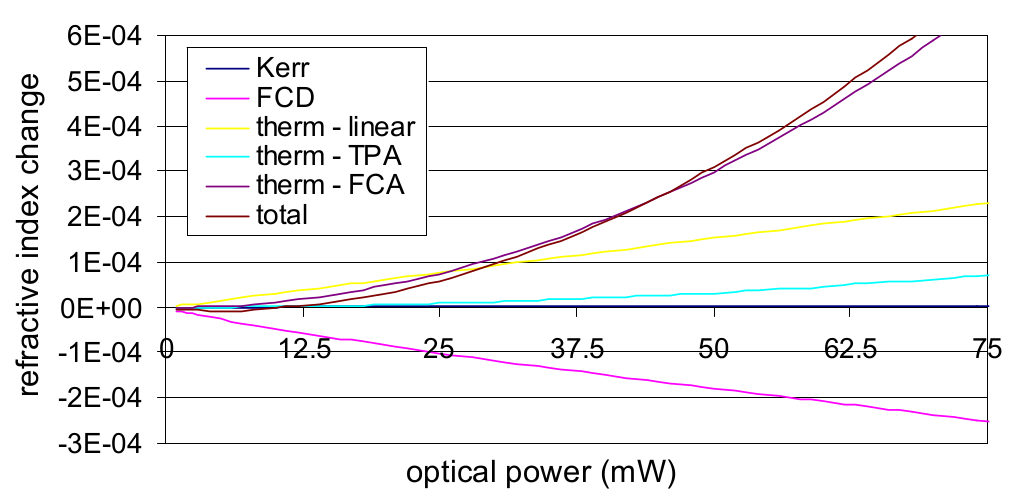
\includegraphics[scale=.5]{figures/Baets_NL_dependence.png}\\
	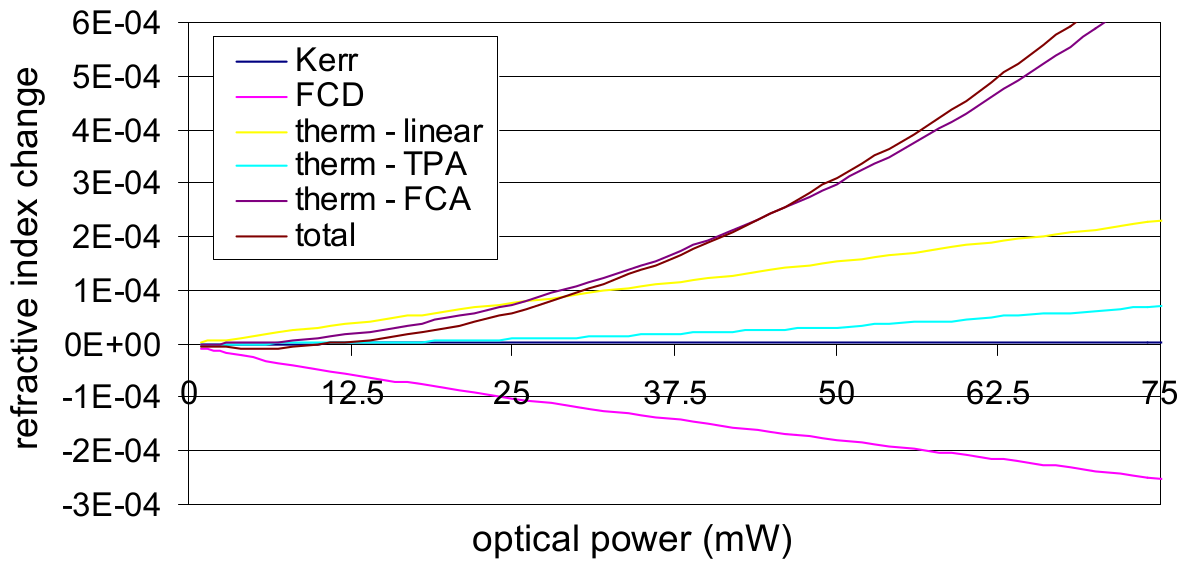
\includegraphics[scale=.4]{figures/Baets_NL_dependence_400.png}
	\caption{Nonlinear contributions to the refractive index change inside the ring res-
onator as function of the cavity power, taken from \cite{priem2005optical}.}
	\label{fig:NL_effects}
\end{figure}

When injecting light into a resonator, its transfer function ultimately depends on two factors: the frequency of the light compared to the frequency of the resonance and the optical power injected.
At low intensities the response of a microring to frequencies around its resonance is symmetrical, as was shown in the preceding section.
At higher intensities, however, the nonlinear phenomena change the refractive index of the material so much that the resonance frequency shifts.
Not all nonlinear mechanisms act in the same way: for example, thermal and FCD phenomena have opposed and competing effects, which shift the resonance in opposite directions.
However, as already stated, on long timescales thermal nonlinearities predominates over all the others.
Hence, after the system has reached the quasi-static regime, as the intensity of the input beam grows, the cavity heats up and the refractive index increases.
This produces a shift of the \textit{cold} resonance towards smaller frequencies, as shown in \autoref{fig:NL_resonance}.
%, where there are two responses perturbed by a shift of $\Delta n=\num{1e-3}$ and $\Delta n=\num{1e-3}$ respectively.

\begin{figure}[hbtp]
	\centering
	\tikzsetexternalprefix{tikz/}	% set subfolder
\tikzsetnextfilename{NL_resonance}
\begin{tikzpicture}[baseline]
	\newcommand\CENTRAL{192}
	\newcommand\START{190.9}
	\newcommand\STOP {193}
	\newcommand\CC{299792458}
	
	\begin{axis}[
			axis x line*= bottom,
			xlabel = {Optical Frequency $\nu$ [$\si{\THz}$]},
			ylabel = {Transmission},
			legend columns=-1,
			legend cell align=right,
			legend style={ at={(0.5,-0.22)}, anchor=north },
			width=\textwidth*0.75,%
			height=207pt,
			xmin= 190.95, xmax = 193,
			%
			% global plot definition
			domain = \START:\STOP,
			samples = 101,
			smooth,
			no markers,
			cycle multi list={
%					exotic
					blue, orange, red
				},
			]
				
		\foreach \TA/\LA/\Radius/\Neff in {0.85/0.9/5/3.826, 0.85/0.9/5/3.827, 0.85/0.9/5/3.830 }{
			\edef\temp{
				\noexpand\addlegendimage{empty legend}
				\noexpand\addlegendentry{$n_{eff}=\Neff:$};
				\noexpand\addplot 
										{ + (1-\TA^2)^2 * \LA
											/ ( (1-\TA^2 * \LA)^2 	+ 4 * \TA^2 	* \LA *sin(deg(\Neff*pi*\Radius*2*pi*x*1e6/\CC))^2 )
										};
				\noexpand\addlegendentry{$D(\omega)$};
%				\noexpand\addplot 
%										{ + \TA^2 * ( (1- \LA)^2	+ 4 					* \LA *sin(deg(\Neff*pi*\Radius*2*pi*x*1e6/\CC))^2 )
%											/ ( (1-\TA^2 * \LA)^2 	+ 4 * \TA^2 	* \LA *sin(deg(\Neff*pi*\Radius*2*pi*x*1e6/\CC))^2 )
%										};
%				\noexpand\addlegendentry{$T(\omega)$};
				}
			\temp
		}
		
		\node [draw=black, fill=white, align=center] at (192.7,0.5) {$\tau=0.85$\\ $\gamma=0.9$\\ $R=\SI{5}{\um}$};
		
	\end{axis}
	
	\begin{axis}[
			width=\textwidth*0.75,%
			height=207pt,
			axis x line*= top,
			axis y line = none,
			xlabel = {Wavelength $\lambda$ [\si{\nm}]},
			samples=2,
			xmin= 190.95, xmax = 193,
			xtick = {193.41448903, 193.16524356, 192.91663964, 192.66867481, 192.421, 192.17465256, 191.92859027, 191.68315729, 191.43835121, 191.19416964, 190.95061019},
			scaled x ticks = manual:{}{ \pgfkeys{/pgf/fpu}\pgfmathparse{(1e-3*\CC/#1)} },
			/pgf/number format/1000 sep=,
		]
		\addplot[white, only marks] coordinates {(191,0.3) (192.95, 0.3)};
	\end{axis}
	
\end{tikzpicture}
	\caption{Microring resonator optical response in three different conditions: unaltered (blue), slightly increased $\Delta n=\num{1e-3}$ (orange), and substantially increased $\Delta n=\num{1e-2}$ refractive index (red).
	Both changes simulates the nonlinear effect of (mostly) thermal nonlinearities.}
	\label{fig:NL_resonance}
\end{figure}

This means that by injecting a certain (high) optical power at higher frequency than the resonance frequency, or on the blue shoulder of the resonance, the obtained transmission will be higher than the one described by the linear equations.
On the other hand, by injecting the same amount of optical power at lower frequency, or on the red shoulder of the resonance, the resulted transmission will be lower than the one described by the linear equations.

\begin{figure}[htbp]
	\begin{subfigure}[b]{0.49\textwidth}
		\centering
		\tikzsetexternalprefix{tikz/}	% set subfolder
\tikzsetnextfilename{OpticalLimiting}
\begin{tikzpicture}[baseline]
	\begin{axis}[
			xlabel={Input optical power},
			ylabel={Output optical power},
			xtick={0},
			ytick={0},
		]
		\newcommand\LIM{10}
		\addplot [black!50, 	domain=0:7.5,		samples=101, smooth, dashed]	{x};
		\node [below left, align=center] at (6,7.5) {\footnotesize maximum\\ \footnotesize transmission\\ \footnotesize line};
		\addplot [blue, 	domain=0:\LIM,		samples=101, smooth]	{x*exp(-5e-2*x)};
	\end{axis}
\end{tikzpicture}
		\caption{Optical limiting}
		\label{fig:optical_limiting_example}
  \end{subfigure}
  \begin{subfigure}[b]{0.49\textwidth}
  		\centering
		\tikzsetexternalprefix{tikz/}	% set subfolder
\tikzsetnextfilename{OpticalBistabilityExample}
\begin{tikzpicture}[baseline]
	\begin{axis}[
			xlabel={Input optical power},
			ylabel={Output optical power},
			xtick={0},
			ytick={0},
		]
		\newcommand\LIM{10}
		\addplot [name path=upwards, blue, 	domain=0:\LIM,		samples=101, smooth, thick]
			{.2*x+(.1+exp(-1e1*(x-7)))^-1};
		\addplot [name path=downwards, red, 	domain=0:\LIM,		samples=101, smooth, thick, dashed]
			{.2*x+(.1+exp(-1e1*(x-3)))^-1};
			
		\addplot [pattern color=gray!25, pattern=north west lines] fill between [
			of=upwards and downwards,
			soft clip={domain=2:8},
		];
		
		\node [fill=white, align=center] at (5.25,5.5)	 {\footnotesize bistability\\\footnotesize region};
		
		\draw [-stealth, blue] (2.25,-0.1) -- (3.25,0.1);
		\draw [-stealth, red ] (8.1,12.2) -- (7.1,12.0);
		
		\node at (6.75,2) [pin={[pin edge={blue}]right:{\scriptsize low half}}] {};
		\node at (3.7,10) [pin={[pin edge={red}]left:{\scriptsize high half}}] {};
		
	\end{axis}
\end{tikzpicture}
		\caption{Optical bistability}
		\label{fig:bistability_example}
  \end{subfigure}
  \caption{
		Examples of (a) optical limiting and (b) optical bistability.
		These curves are just a qualitative example of the phenomena.
		More accurate representation will be shown in the \autoref{ssec:Simulations}.
  }
  	\label{fig:nonlinear_examples}
\end{figure}

These features can be exploited to obtain two different effects.
By choosing a signal with a fixed frequency on the blue shoulder of the \textit{cold} resonance, the effect obtained is \textit{optical limiting}.
Optical limiting is the progressive decrease in transmission with the increase of the input signal.
Hence, the effective transmission produced is nonlinearly dependent on the value of the input signal, as shown in \autoref{fig:optical_limiting_example}.
On the other hand, by choosing a signal on the red shoulder of the \textit{cold} resonance, the effect obtained is \textit{optical bistability}.
Optical bistability is the existence of two distinct steady states of the transmission function for the same interval of input signals.
In an optical microring resonator this produces abrupt \textit{jumps} from one steady state to the other, when at the edges of such intervals.
Specifically, at the right edge of the bistability region, the systems switches from the lower to the higher transmission state, whereas at the left edge, the system switches from the higher to the lower tramsission state.
Moreover, the state inside the bistability interval is determined by the past states of the optical cavity.
This defines a hysteresis cycle around the bistability region.
All these features are shown in \autoref{fig:bistability_example}.

\clearpage
\section{Integrated photonics applied to ANNs}
\label{sec:Integrated_photonics_applied_to_ANNs}
Even though the vast majority of hardware architectures for artificial neural networks are developed within the electronic platform, integrated photonics is emerging as a fast and efficient alternative.
The way in which information is elaborated inside neural networks seems to be more favorable, in comparison to the boolean logic, to the development of photonic integrated processors \cite{shastri2017emergence}.
The aim of photonics is to match the performances of electronics in the development of neuromorphic networks by exploiting its inherent suitability to parallel computing, its bandwidth and speed, and also its power efficiency (see \autoref{tab:neuromorphic_arc}).

\begin{table}[!htbp]
	\centering
	\footnotesize
	\begin{tabular}{l r r r r}
	\toprule
	\normalsize Chip & \normalsize MAC rate & \normalsize Energy per MAC & \normalsize Area per MAC \\
	& & (\si{\pico\joule}) & (\si{\square\um})\\
	\midrule
	Photonic hybrid III-V/Si & \SI{20}{\GHz} & \num{1.3} 	& 205 \\
	Sub-$\lambda$ photonics (future trend) & \SI{200}{\GHz} & \num{0.0007} 	& 20 \\
	HICANN & \SI{22.4}{\MHz} & \num{198.4} 	& 780 \\
	TrueNorth & \SI{2.5}{\kHz} & \num{0.27} 	& 4.9 \\
	Neurogrid & \SI{40.1}{\kHz} & \num{119} 	& 7.1 \\
	SpiNNaker & \SI{3.2}{\kHz} & \num{6e5} 	& 217 \\
	\bottomrule
	\end{tabular}
	\caption{Comparative table on current and future trends in electronic and photonic micro-architectures for neuromorphic computing. MAC stands for \textit{Multiply and ACcumulate} operation, a standard computational step. Taken from \cite{de2017progress}.}
	\label{tab:neuromorphic_arc}
\end{table}

Nevertheless building a neural network within a photonic integrated chip is a demanding task.
For this reason, the results achieved until now have been obtained by using a small number of integrated devices.
This fact inevitably limits the maximum complexity of the neural networks built.
However, many neuromorphic networks are based on the reservoir computing (RC) approach or the recurrent neural network (RNN) type or both.
The first one is a learning method that allows to have little to no control on the majority of the network while employing all efforts on the training of a single output layer \cite{van2017advances, haynes2015reservoir}.
Hence very fast and complex system can be exploited without having real control on the local effects that happen inside the \textit{reservoir}.
On the other hand, a recurrent neural network can be implemented with only one computational node \cite{dejonckheere2014all, haynes2015reservoir}, as it exploit time to distribute the computation.
In this type of network, the lack of physical complexity is compensated by the extension in time of the required task.

The idea of this work is to tackle the problem head on and develop a framework for feedforward artificial neural network based on optical effects.
%In this section, I will describe the fundamental ideas at the base of my photonic implementation of a neural network.
%The optical microring resonator, specifically in the ADF configuration, is the hardware on which my implementation is based.
%Since the response of this type of resonators is multifaceted, as many physical quantities can be used as input or output variables, I will explain precisely how its response will be used.
%Thus, I will make wide use of the theoretical base illustrated in the earlier sections, specifically on the nonlinear effects.

As shown in \autoref{sec:Basis_of_Neural_Networks}, the principal parts of an artificial neural network are its nodes, which in turn are built by two separate subcomponents: the weighted sum and the nonlinear activation function.
%In the next sections I will describe some photonic devices that have been developed to perform those tasks, along with my implementation of an all-optical nonlinear activation function with a microring resonator.
In the next sections I will describe how the nonlinear response of a microring could be exploited in an all-optical node of a feedforward ANN.

\subsection{Weighted sum of inputs}
\label{ssec:Weighted_Sum_of_inputs}
The difficulty in the weighted sum of inputs does not lie in the type of operation, i.e. sum and multiplication, but in the fact that each node has many inputs.
Excluding the cases in which the weighted summation has been carried off by online or offline elaboration on standard computers, there are two important examples of all-optical weighted sum.

The first one \cite{Shen2017} is based on a cascade of Mach-Zehnder Interferometers (MZI), which transforms all the outputs of a whole layer to the set of inputs of the next one.
This happens by a sequence of constructive and destructive interferences that alter the starting coherent signal.

The second example \cite{Tait2017} is given by a series of microring resonator, parametrically tuned to transmit a portion of light.
In this work, different signals are multiplexed on many wavelengths and are weighted by consecutive rings built in such a way that they affects only a certain wavelength.
Moreover, the weight is implemented by thermal finetuning of the resonator cavities.
This example, however, exploit an optoelectronic nonlinear stage composed of two photodiodes and a light source nonlinearly dependent to the current produced by the photodiodes.

\subsection{Nonlinear Activation Function}
\label{ssec:Nonlinear_Activation_Function}
The development of novel optical mechanisms for the nonlinear activation function in ANNs has not progressed as much as the development of the weighted sum of the node inputs has.
%As opposed to the mechanism for weighted sum, optical phenomenon for the activation function in an integrated photonic circuit has not been discussed much.
In fact, many proposed PICs by means of integrated optical structures realize the weighting part of the inputs only.
The nonlinear activation function is then implemented either by electronic devices \cite{Tait2017} or even by computer aided evalutation \cite{Shen2017}.

An interesting proposal is to employ a saturable absorber to obtain a nonlinear activation function \cite{dejonckheere2014all}.
Saturable absorbers are materials that have a reduced absorption of light for high optical intensities.

The idea of my work is to employ the optical bistability in a microring resonator as a mean to obtain a nonlinear activation function, that simulate the commonly used sigmoid one.
Optical bistability, as seen in \autoref{ssec:Nonlinear_perturbation_of_microring_response}, is an optical effect that occurs when injecting light in a microring resonator with a lower frequency in respect to the resonance frequency.

In a quasi-static regime, optical bistability is mainly due to the therm-optic effect, which depends from the temperature.
However, temperature depends in turn from the optical power circulating inside the cavity, which is obviously determined by the input intensity.
This allows to obtain a total output transmission that depends nonlinearly on the input intensity.

\subsection{Simulations}
\label{ssec:Simulations}
In order to better understand the physical mechanisms underneath the microring behavior, I used numerical methods to simulate the response of a microring resonator.
Since the experiments are carried out in the quasi-static regime, the system can be described by a set of three coupled algebraic equations: one for the enhancement factor, one for the free carrier dynamics, and one for the thermal dynamics.

\begin{align}
EF \left( \omega \right)
	&= \dfrac	{ \gamma \Delta\gamma}
		{ \left( 1-\tau^2	\gamma \Delta\gamma \right)^2 + 4 \tau^2	\gamma \Delta\gamma \sin^2 \left( \left(n_{eff} + \Delta n_{eff}\right) \frac{\omega}{c_0} \pi R \right) }\\
\Delta N
	&= \frac{1}{\gamma_{FC}} \frac{\beta_{TPA}}{2\hbar \omega} I^2\\
\Delta T
	&= \frac{1}{\gamma_{TH}}\frac{1}{M_{ring}C_p} V\left(\alpha_{eff} + \beta_{TPA} I + \dfrac{d\alpha}{dN} \Delta N \right) I
\end{align}
where
\begin{align}
I 								&= EF~I_{input}\\
\Delta\gamma 		&= e^{-\left(\beta_{TPA} I + \frac{d\alpha}{dN} \Delta N \right) \pi R }\\
\Delta n_{eff} 	&= n_2 I + \frac{dn}{dN} \Delta N + \frac{dn}{dT} \Delta T
\end{align}

This set of equations allows a simple but complete description of the physical quantities of interest in the system.

To decrease numerical errors, a reduced variable approach has been used.
This means that every factor in the equations has been divided by the order of magnitude typical of the problem, to reduce or increase its numerical representation towards unity.
For examples, distances have been reduced to \si{\um} and powers to \si{\mW} and so on.

In addition, important values that are not explicitly computed, such as the transmission of the through and drop channels, can be extracted with just a simple multiplication.
Moreover, adding another light source at a different wavelength (or frequency) is very simple.
It is obtained by adding a second equation for the enhancement factor $EF(\omega_2)$ and by redefining the optical intensity circulating inside to $I = EF\left(\omega_1\right)I_{input}\left(\omega_1\right) + EF\left(\omega_2\right)I_{input}\left(\omega_2\right)$.
This neglects interference effects between the two beams, but then again the whole evaluation is a first-order-approximation.
%Besides, interference effect are limited in the most interesting case which is the \textit{pump-and-probe}, where a beam has much higher intensity (pump) in comparison to the other beam (probe).

To obtain the correct values that verifies the set of equations, I employed an iterative algorithm.
First of all I assume a certain set of initial conditions for $EF$, $\Delta N$, and $\Delta T$, which I will call $\left.EF\right|_0$, $\left.\Delta N\right|_0$, and $\left.\Delta T\right|_0$ respectively.
For example one could choose to start from a \textit{cold} system by setting them to zero.
Then I evaluate the values the same variable at the next step by parametrically replacing the variables with their newly discovered values.
\begin{align*}
1) \qquad &\left.EF\right|_1=EF(\omega,\left.EF\right|_0,\left.\Delta N\right|_0,\left.\Delta T\right|_0) \\
2) \qquad &\left.\Delta N\right|_1 = \Delta N(\left.EF\right|_1,\left.\Delta N\right|_0,\left.\Delta T\right|_0) \\
3) \qquad &\left.\Delta T\right|_1 = \Delta N(\left.EF\right|_1,\left.\Delta N\right|_2,\left.\Delta T\right|_0)
\end{align*}
which is easily generalized by putting $\left.\right|_0 \rightarrow \left.\right|_n$ and $\left.\right|_1 \rightarrow \left.\right|_{n+1}$.
These three steps must be repeated until they converge to a steady state value.
%the values obtained gradually improve toward the correct ones.
%A simple check on this condition, or on a maximum number of iterations, exits the loop.

At low input intensities nonlinearities are negligible, thus the output has the shape of the \textit{cold} resonance, as shown in \autoref{fig:sim_cold_resonance}.

\begin{figure}[htbp]
	\centering
	\tikzsetexternalprefix{tikz/}	% set subfolder
\tikzsetnextfilename{cold_resonance}

\begin{tikzpicture}[baseline]

	\definecolor{color1}{rgb}{0.12156862745098,0.466666666666667,0.705882352941177}
	
	\begin{axis}[
			title={Internal Power},
			xlabel={Wavelength distance $\Delta\lambda$ [\si{\nm}]},
			ylabel={Internal Power [arb.units]},
			tick align=outside,
			tick pos=left,
			width=\textwidth*0.75,%
			height=207pt,
			legend pos = outer north east,
			/pgf/number format/1000 sep=,
		]
		\addlegendentry{\hspace{-.6cm}$P_{input}$}
		\addlegendimage{empty legend};
		
    \addplot [semithick, color1, mark=*, mark size=1, mark options={solid}]
    		table [x index=0, y index=1] {tikz/triangles.csv};
   	\pgfplotstableread{tikz/triangles.csv}\table 
		\pgfplotstablegetcolumnnamebyindex{1}\of{\table}\to{\colname}
    \addlegendentryexpanded{ \SI{\colname}{\mW}}
    
	\end{axis}
\end{tikzpicture}
	\caption{
		Shape of the resonance when probed with a low intensity signal.
		As expected is a lorentzian-type of curve, like in \autoref{fig:ADF}.
	}
	\label{fig:sim_cold_resonance}
\end{figure}

At higher intensities the nonlinear effects become non negligible and therefore the number of iteration required increases.
The algorithm evolution follows the same steps of the physical system: the system start off in a \textit{cold} state and the gets progressively heated by the light that gets coupled inside the cavity.
%The sequential way with which this happens is a common trait for both the algorithm and the physical system.

However, the optical bistable region is also a region of instability for the algorithm, because there are two stable and infinite unstable states.
As for the physical system, which selects the state depending on the past condition of the cavity, the same happens for the algorithm.
By choosing as initial conditions the output values of the the variables obtained by the evaluation of the previous set of parameters, proved to be a successful approach to the problem.

Still, this method is not enough at high intensities, when the algorithm could not reach a steady state value due to the high number of iterations required.
This is due to the fact that in certain regions, the values of consequent iterations oscillate around the steady state without any tangible progress toward convergence.
This drastically increases the number of iteration required.
For this reason I modified the algorithm from the vanilla iteration above to a more complex one.
In this revised algorithm the variables at each new step are evaluated with a mix of the last and second to last values instead of just the last one.
This method contrasts the phenomenon of uncontrolled value oscillation.
%I heuristically found that 

The results of the algorithm, for input parameters given by a sequence of signals of increasing optical power at a precise distance from the resonance wavelength, map half of the hysteresis cycle.
It is important in this case to set the initial conditions as the output values of the last evaluated state.
Similarly, by setting the input parameters with a sequence of signals of decreasing optical power, the results map the other half of the bistability hysteresis cycle.
The collection of the outcomes, obtained by repeating this evaluations for a set of different wavelengths on the red shoulder of the resonance, is shown in \autoref{fig:sim_bist_cycle}.

\begin{figure}[ht]
	\centering
%	\tikzsetexternalprefix{tikz/}	% set subfolder
\tikzsetnextfilename{bistability_test}
% This file was created by matplotlib2tikz v0.6.15.
\begin{tikzpicture}[baseline]
	
	\pgfplotstableread[col sep=tab, header=true]{tikz/foo.csv}\loadedtable
	
	\pgfplotstablegetcolsof{\loadedtable}
	\pgfmathparse{\pgfplotsretval - 1}
	\newcommand{\ncol}{\pgfmathresult}
	
	\definecolor{color1}{rgb}{1,0.498039215686275,0.0549019607843137}
	\definecolor{color6}{rgb}{0.890196078431372,0.466666666666667,0.76078431372549}
	\definecolor{color5}{rgb}{0.549019607843137,0.337254901960784,0.294117647058824}
	\definecolor{color2}{rgb}{0.172549019607843,0.627450980392157,0.172549019607843}
	\definecolor{color4}{rgb}{0.580392156862745,0.403921568627451,0.741176470588235}
	\definecolor{color3}{rgb}{0.83921568627451,0.152941176470588,0.156862745098039}
	\definecolor{color0}{rgb}{0.12156862745098,0.466666666666667,0.705882352941177}

\begin{axis}[
		title={Internal Power},
		xlabel={Pump Power $P$ $[mW]$},
		ylabel={Internal Power [a.u.*]},
		xmin=0.852408771935031, xmax=4.09941578936435,
		ymin=-3215.6821653405, ymax=90671.1511338174,
		tick align=outside,
		tick pos=left,
		width=\textwidth*0.75,%
		height=207pt,
		%x grid style={lightgray!92.02614379084967!black},
		%y grid style={lightgray!92.02614379084967!black},
		legend entries={
			{$\Delta\lambda$},
			{\SI{350}{\pm}},
			{\SI{379}{\pm}},
			{\SI{407}{\pm}},
			{\SI{436}{\pm}},
			{\SI{464}{\pm}},
			{\SI{493}{\pm}},
			{\SI{521}{\pm}},
			{\SI{550}{\pm}}
			},
		legend pos = outer north east,
		%legend cell align={left},
		%legend style={at={(1,-0.1)}, anchor=north west, draw=white!80.0!black},
		%legend columns=8
	]
	
	\addlegendimage{empty legend}
	\addlegendimage{mark=*, color0}
	\addlegendimage{mark=*, color1}
	\addlegendimage{mark=*, color2}
	\addlegendimage{mark=*, color3}
	\addlegendimage{mark=*, color4}
	\addlegendimage{mark=*, color5}
	\addlegendimage{mark=*, color6}
	\addlegendimage{mark=*, gray!99.6078431372549!black}

%\addlegendentry = {$\Delta\lambda$}
%\addlegendimage = {empty legend}
%\foreach \i in {1,2...,\pgfplotsretval-1} {
%	\addplot table [x index=0, y index=\i] {\loadedtable};
%	\pgfplotstablegetcolumnnamebyindex{\i}\of{\loadedtable}\to\colname
%	\addlegendentry = {\SI{\colname}{\pm}}
%	\addlegendimage = {mark=*, color\i}
%}

\addplot [semithick, color0, mark=*, mark size=1, mark options={solid}]
table {%
1 2182.13784798453
1.10996151344182 2732.06812562319
1.20997071148193 3301.35802903992
1.30232241935941 3891.75515464847
1.38854537026638 4505.26943967214
1.46971861477299 5144.22980210166
1.54663743906977 5811.35713826561
1.61990800024395 6509.85972553239
1.69000487886171 7243.55987029429
1.75730789900303 8017.0649998584
1.82212667320922 8836.00339261668
1.88471753176505 9707.35631717665
1.94529553946556 10639.9381155571
2.00404323735458 11645.110858216
2.06111713847338 12737.8851497554
2.11665264505793 13938.6847549387
2.1707678321628 15276.31091276
2.22356640163383 16793.2014266478
2.27514001850367 18555.3533357662
2.32557018064795 20672.1913566021
2.37492973084278 23336.6084050299
2.42328409142697 26875.9830526321
2.47069228134243 31476.9310455102
2.51720776067593 36046.2694806532
2.56287913716765 39544.1852080518
2.60775076129818 42181.9936544263
2.65186323070653 44282.0696014857
2.69525382027284 46032.9554507758
2.73795685083191 47541.7982041075
2.78000400689269 48873.3912118438
2.82142461172746 50069.4947595316
2.86224586662004 51158.5039921599
2.9024930598204 52160.5856929643
2.94218974976591 53090.5802810476
2.98135792633989 53959.7327474007
3.02001815330168 54776.7742586017
3.05818969450781 55548.625360946
3.09589062612293 56280.8689540435
3.13313793667592 56978.0778524274
3.16994761653247 57644.0474967912
3.20633473812108 58281.9649496754
3.24231352805431 58894.5341847922
3.27789743212414 59484.0704107321
3.31309917401337 60052.5723212442
3.34793080845022 60601.7782354623
3.38240376943561 61133.2101736674
3.41652891409018 61648.2089375426
3.45031656259774 62147.9622831466
3.48377653466154 62633.5277873525
3.51691818283855 63105.8515562808
3.54975042307237 63565.7836494865
3.58228176270719 64014.090916815
3.61452032623231 64451.4677214149
3.64647387897796 64878.5449862339
3.67814984895812 65295.8978439847
3.70955534703456 65704.052169585
3.74069718555709 66103.4901635271
3.77158189561844 66494.655157941
3.80221574304758 66877.9557805134
3.83260474325241 67253.7695572549
3.86275467501147 67622.4460626382
3.89267109330405 67984.3096727404
3.92235934125968 68339.6619855259
3.95182456129939 68688.7839488388
};
\addplot [semithick, color1, mark=*, mark size=1, mark options={solid}]
table {%
1 1940.07544411095
1.10996151344182 2423.22716305164
1.20997071148193 2920.70721201128
1.30232241935941 3433.61186262683
1.38854537026638 3963.17696183345
1.46971861477299 4510.8034528873
1.54663743906977 5078.08911859356
1.61990800024395 5666.86848769019
1.69000487886171 6279.26358787269
1.75730789900303 6917.74933289089
1.82212667320922 7585.2389829278
1.88471753176505 8285.19764576196
1.94529553946556 9021.7957820453
2.00404323735458 9800.12113436134
2.06111713847338 10626.4782986138
2.11665264505793 11508.8239192492
2.1707678321628 12457.4194811703
2.22356640163383 13485.848418119
2.27514001850367 14612.6752996465
2.32557018064795 15864.3096818447
2.37492973084278 17280.3143272715
2.42328409142697 18924.1988617378
2.47069228134243 20908.2895226999
2.51720776067593 23462.0392880969
2.56287913716765 27170.8381037511
2.60775076129818 33631.0297137638
2.65186323070653 40341.9479641702
2.69525382027284 44189.4013634534
2.73795685083191 46803.6856546889
2.78000400689269 48821.2416782276
2.82142461172746 50486.4792493101
2.86224586662004 51917.3882993097
2.9024930598204 53180.0763622241
2.94218974976591 54315.4654194578
2.98135792633989 55350.7465285369
3.02001815330168 56304.9665061537
3.05818969450781 57192.0231155222
3.09589062612293 58022.3918927019
3.13313793667592 58804.1805477364
3.16994761653247 59543.8034465492
3.20633473812108 60246.430206525
3.24231352805431 60916.2935960542
3.27789743212414 61556.9070656952
3.31309917401337 62171.2219851855
3.34793080845022 62761.7437447084
3.38240376943561 63330.6190515937
3.41652891409018 63879.7026494471
3.45031656259774 64410.6090421554
3.48377653466154 64924.7531439948
3.51691818283855 65423.3825577898
3.54975042307237 65907.6035338806
3.58228176270719 66378.4020054886
3.61452032623231 66836.6608209025
3.64647387897796 67283.1739473754
3.67814984895812 67718.6582859319
3.70955534703456 68143.7635642359
3.74069718555709 68559.0806667746
3.77158189561844 68965.1487014138
3.80221574304758 69362.4610174769
3.83260474325241 69751.4703637162
3.86275467501147 70132.5933346228
3.89267109330405 70506.2142143482
3.92235934125968 70872.6883067225
3.95182456129939 71232.3448615192
};
\addplot [semithick, color2, mark=*, mark size=1, mark options={solid}]
table {%
1 1732.97280209881
1.10996151344182 2160.25082035293
1.20997071148193 2598.25542831804
1.30232241935941 3047.68385058352
1.38854537026638 3509.3086372655
1.46971861477299 3983.98931489536
1.54663743906977 4472.68642687737
1.61990800024395 4976.47859191022
1.69000487886171 5496.5834020755
1.75730789900303 6034.38326074926
1.82212667320922 6591.45765894542
1.88471753176505 7169.62394084324
1.94529553946556 7770.98943472775
2.00404323735458 8398.01903253042
2.06111713847338 9053.62415924678
2.11665264505793 9741.28193834583
2.1707678321628 10465.1979664045
2.22356640163383 11230.5337188335
2.27514001850367 12043.7326151105
2.32557018064795 12913.002021987
2.37492973084278 13849.0520482085
2.42328409142697 14866.2785935804
2.47069228134243 15984.7629825415
2.51720776067593 17233.8916436386
2.56287913716765 18659.5263921909
2.60775076129818 20340.0938776341
2.65186323070653 22430.0792057072
2.69525382027284 25321.8960673326
2.73795685083191 30987.8016123129
2.78000400689269 44888.9927766667
2.82142461172746 48918.4586028915
2.86224586662004 51428.5184753255
2.9024930598204 53337.2501195886
2.94218974976591 54909.1358036994
2.98135792633989 56261.2528516411
3.02001815330168 57456.8190350748
3.05818969450781 58534.2614456403
3.09589062612293 59518.8696435552
3.13313793667592 60428.26786974
3.16994761653247 61275.282136951
3.20633473812108 62069.5689773745
3.24231352805431 62818.6003117727
3.27789743212414 63528.2893700834
3.31309917401337 64203.4049985116
3.34793080845022 64847.8553330121
3.38240376943561 65464.8876903212
3.41652891409018 66057.2328970549
3.45031656259774 66627.2118303121
3.48377653466154 67176.8154208414
3.51691818283855 67707.7658504522
3.54975042307237 68221.5639803765
3.58228176270719 68719.5266349635
3.61452032623231 69202.8162397473
3.64647387897796 69672.4646422314
3.67814984895812 70129.3924540031
3.70955534703456 70574.4248816071
3.74069718555709 71008.3048010219
3.77158189561844 71431.7036445875
3.80221574304758 71845.2304972518
3.83260474325241 72249.4397994264
3.86275467501147 72644.8378492904
3.89267109330405 73031.8883777777
3.92235934125968 73411.0173027476
3.95182456129939 73782.6168527726
};
\addplot [semithick, color3, mark=*, mark size=1, mark options={solid}]
table {%
1 1555.12712962575
1.10996151344182 1935.35022328765
1.20997071148193 2323.70064537386
1.30232241935941 2720.62917693881
1.38854537026638 3126.62808241723
1.46971861477299 3542.23655447464
1.54663743906977 3968.04710570885
1.61990800024395 4404.71310972971
1.69000487886171 4852.95775950785
1.75730789900303 5313.58477279263
1.82212667320922 5787.49128427383
1.88471753176505 6275.68348806087
1.94529553946556 6779.2957771205
2.00404323735458 7299.61438270963
2.06111713847338 7838.1068655017
2.11665264505793 8396.45931641251
2.1707678321628 8976.62387064854
2.22356640163383 9580.88022625359
2.27514001850367 10211.916530394
2.32557018064795 10872.9375886795
2.37492973084278 11567.812506292
2.42328409142697 12301.2807338782
2.47069228134243 13079.2472517646
2.51720776067593 13909.2186734183
2.56287913716765 14800.9715720034
2.60775076129818 15767.623259535
2.65186323070653 16827.4446215626
2.69525382027284 18007.1530903572
2.73795685083191 19348.4800019746
2.78000400689269 20923.1011850703
2.82142461172746 22874.1137116357
2.86224586662004 25581.679254139
2.9024930598204 32373.8833560084
2.94218974976591 53685.3764633791
2.98135792633989 56034.1288896655
3.02001815330168 57820.9838468359
3.05818969450781 59297.9114358345
3.09589062612293 60573.1864351054
3.13313793667592 61704.6888586915
3.16994761653247 62727.4816976698
3.20633473812108 63664.6266831185
3.24231352805431 64532.2068880532
3.27789743212414 65341.9425439077
3.31309917401337 66102.6722811745
3.34793080845022 66821.2474128613
3.38240376943561 67503.0999560958
3.41652891409018 68152.6186366019
3.45031656259774 68773.406464817
3.48377653466154 69368.4623655541
3.51691818283855 69940.3124659625
3.54975042307237 70491.1070517066
3.58228176270719 71022.6935267439
3.61452032623231 71536.6722322788
3.64647387897796 72034.4397820577
3.67814984895812 72517.2231554371
3.70955534703456 72986.1068373264
3.74069718555709 73442.0546571947
3.77158189561844 73885.9275378199
3.80221574304758 74318.4980334294
3.83260474325241 74740.4623689852
3.86275467501147 75152.4504450848
3.89267109330405 75555.034238381
3.92235934125968 75948.7348944082
3.95182456129939 76334.028743014
};
\addplot [semithick, color4, mark=*, mark size=1, mark options={solid}]
table {%
1 1401.7392420467
1.10996151344182 1742.05447923165
1.20997071148193 2088.60129970629
1.30232241935941 2441.67621144985
1.38854537026638 2801.59908560004
1.46971861477299 3168.71577477143
1.54663743906977 3543.40111578359
1.61990800024395 3926.06239167527
1.69000487886171 4317.14333702743
1.75730789900303 4717.12879862109
1.82212667320922 5126.55018167644
1.88471753176505 5545.99185421269
1.94529553946556 5976.0987168996
2.00404323735458 6417.58521344896
2.06111713847338 6871.24612225125
2.11665264505793 7337.96958510755
2.1707678321628 7818.75295467511
2.22356640163383 8314.72224806523
2.27514001850367 8827.15625233288
2.32557018064795 9357.51670762848
2.37492973084278 9907.48654853509
2.42328409142697 10479.0189765846
2.47069228134243 11074.4013469418
2.51720776067593 11696.3396961176
2.56287913716765 12348.0726453624
2.60775076129818 13033.5281305727
2.65186323070653 13757.5443237197
2.69525382027284 14526.1899146087
2.73795685083191 15347.2441508942
2.78000400689269 16230.9456576159
2.82142461172746 17191.2192207557
2.86224586662004 18247.8134492887
2.9024930598204 19430.3365989971
2.94218974976591 20786.7549552248
2.98135792633989 22404.3765552702
3.02001815330168 24477.132776658
3.05818969450781 27686.4341351164
3.09589062612293 60604.7367382226
3.13313793667592 62267.3306556756
3.16994761653247 63651.8767800161
3.20633473812108 64854.0003360527
3.24231352805431 65925.1989624745
3.27789743212414 66896.8638024415
3.31309917401337 67789.7512506825
3.34793080845022 68618.4032399159
3.38240376943561 69393.4596711254
3.41652891409018 70122.9731701597
3.45031656259774 70813.2057695201
3.48377653466154 71469.1366375532
3.51691818283855 72094.7992028596
3.54975042307237 72693.5127477348
3.58228176270719 73268.04615849
3.61452032623231 73820.7365353523
3.64647387897796 74353.577049637
3.67814984895812 74868.2831356681
3.70955534703456 75366.343267635
3.74069718555709 75849.0584399384
3.77158189561844 76317.5732904656
3.80221574304758 76772.9009091922
3.83260474325241 77215.9428404241
3.86275467501147 77647.5053551995
3.89267109330405 78068.3128118444
3.92235934125968 78479.018719511
3.95182456129939 78880.2149507901
};
\addplot [semithick, color5, mark=*, mark size=1, mark options={solid}]
table {%
1 1268.82868775917
1.10996151344182 1575.05802024631
1.20997071148193 1886.12026197023
1.30232241935941 2202.21379773944
1.38854537026638 2523.5504741739
1.46971861477299 2850.35689401489
1.54663743906977 3182.87587513696
1.61990800024395 3521.36809814379
1.69000487886171 3866.11397301945
1.75730789900303 4217.4157647887
1.82212667320922 4575.60001730141
1.88471753176505 4941.02033443108
1.94529553946556 5314.06057831588
2.00404323735458 5695.1385694657
2.06111713847338 6084.71038352431
2.11665264505793 6483.27536643047
2.1707678321628 6891.38202520844
2.22356640163383 7309.63497755628
2.27514001850367 7738.70321414165
2.32557018064795 8179.32997495534
2.37492973084278 8632.34465296927
2.42328409142697 9098.67724862147
2.47069228134243 9579.37607223338
2.51720776067593 10075.6296358352
2.56287913716765 10588.794003145
2.60775076129818 11120.4273476226
2.65186323070653 11672.3341837221
2.69525382027284 12246.6227764755
2.73795685083191 12845.7808515076
2.78000400689269 13472.7772471925
2.82142461172746 14131.2012233633
2.86224586662004 14825.4579311768
2.9024930598204 15561.0503423298
2.94218974976591 16344.9992760867
2.98135792633989 17186.4940437196
3.02001815330168 18097.9494922264
3.05818969450781 19096.8290326469
3.09589062612293 20209.0416065191
3.13313793667592 21475.970206772
3.16994761653247 22971.3891448233
3.20633473812108 24853.4294810608
3.24231352805431 27628.5741492578
3.27789743212414 67971.5517060323
3.31309917401337 69105.1416733301
3.34793080845022 70120.0946247003
3.38240376943561 71044.1745834219
3.41652891409018 71895.906585186
3.45031656259774 72688.3618266287
3.48377653466154 73431.1596717701
3.51691818283855 74131.6157929157
3.54975042307237 74795.4428143908
3.58228176270719 75427.1994959916
3.61452032623231 76030.5904912877
3.64647387897796 76608.6731994837
3.67814984895812 77164.0045519713
3.70955534703456 77698.7477761974
3.74069718555709 78214.7516479251
3.77158189561844 78713.6104264719
3.80221574304758 79196.7099098472
3.83260474325241 79665.2633847461
3.86275467501147 80120.339956786
3.89267109330405 80562.8872403561
3.92235934125968 80993.7496498591
3.95182456129939 81413.6833305709
};
\addplot [semithick, color6, mark=*, mark size=1, mark options={solid}]
table {%
1 1153.11534113191
1.10996151344182 1430.03226695262
1.20997071148193 1710.73804990963
1.30232241935941 1995.36761972763
1.38854537026638 2284.06383596786
1.46971861477299 2576.97814784539
1.54663743906977 2874.271324898
1.61990800024395 3176.11426828301
1.69000487886171 3482.68891680214
1.75730789900303 3794.18925621961
1.82212667320922 4110.82245204988
1.88471753176505 4432.81012075285
1.94529553946556 4760.38976134927
2.00404323735458 5093.81637550133
2.06111713847338 5433.36430322558
2.11665264505793 5779.32931126422
2.1707678321628 6132.03098200405
2.22356640163383 6491.81544913815
2.27514001850367 6859.0585527477
2.32557018064795 7234.16948577099
2.37492973084278 7617.59503665301
2.42328409142697 8009.82454518515
2.47069228134243 8411.39572435789
2.51720776067593 8822.9015440492
2.56287913716765 9244.9984176772
2.60775076129818 9678.41600447315
2.65186323070653 10123.9690407346
2.69525382027284 10582.5717252035
2.73795685083191 11055.255374458
2.78000400689269 11543.1902961492
2.82142461172746 12047.7131731641
2.86224586662004 12570.3617592033
2.9024930598204 13112.9194050828
2.94218974976591 13677.4730410114
2.98135792633989 14266.4899249147
3.02001815330168 14882.92113088
3.05818969450781 15530.3440849035
3.09589062612293 16213.1637448906
3.13313793667592 16936.9048102428
3.16994761653247 17708.6507936515
3.20633473812108 18537.731333299
3.24231352805431 19436.8536726255
3.27789743212414 20424.0877878307
3.31309917401337 21526.6517346132
3.34793080845022 22789.0048056135
3.38240376943561 24293.3410848102
3.41652891409018 26228.6066943418
3.45031656259774 29348.8257048927
3.48377653466154 75171.1397221552
3.51691818283855 75984.6568808932
3.54975042307237 76743.4666071406
3.58228176270719 77456.2449920176
3.61452032623231 78129.6279619962
3.64647387897796 78768.8222956222
3.67814984895812 79377.9997469359
3.70955534703456 79960.5631547749
3.74069718555709 80519.3292809379
3.77158189561844 81056.6605048151
3.80221574304758 81574.5604661358
3.83260474325241 82074.7454388648
3.86275467501147 82558.6984882122
3.89267109330405 83027.7111994293
3.92235934125968 83482.9163354476
3.95182456129939 83925.3136700693
};
\addplot [semithick, gray!99.6078431372549!black, mark=*, mark size=1, mark options={solid}]
table {%
1 1051.90116643941
1.10996151344182 1303.44726288011
1.20997071148193 1557.99394172329
1.30232241935941 1815.63441347309
1.38854537026638 2076.46666063304
1.46971861477299 2340.59378187961
1.54663743906977 2608.12436994593
1.61990800024395 2879.17292492343
1.69000487886171 3153.86030778706
1.75730789900303 3432.31424093356
1.82212667320922 3714.66985891778
1.88471753176505 4001.07031664975
1.94529553946556 4291.66746463481
2.00404323735458 4586.622597123
2.06111713847338 4886.1072842512
2.11665264505793 5190.30430224765
2.1707678321628 5499.40867237775
2.22356640163383 5813.62882592496
2.27514001850367 6133.18791706005
2.32557018064795 6458.32530267821
2.37492973084278 6789.29821739155
2.42328409142697 7126.38367974316
2.47069228134243 7469.88066200891
2.51720776067593 7820.1125779211
2.56287913716765 8177.43014050562
2.60775076129818 8542.21466092436
2.65186323070653 8914.88187908926
2.69525382027284 9295.88642441276
2.73795685083191 9685.72704972988
2.78000400689269 10084.9527957754
2.82142461172746 10494.1703087648
2.86224586662004 10914.0525718883
2.9024930598204 11345.3494129332
2.94218974976591 11788.9002336084
2.98135792633989 12245.6495758424
3.02001815330168 12716.6663249425
3.05818969450781 13203.1676488722
3.09589062612293 13706.549171899
3.13313793667592 14228.4234937297
3.16994761653247 14770.6700428606
3.20633473812108 15335.5006187596
3.24231352805431 15925.5470950771
3.27789743212414 16543.9811598262
3.31309917401337 17194.6816380418
3.34793080845022 17882.4746784895
3.38240376943561 18613.4896944253
3.41652891409018 19395.7073085347
3.45031656259774 20239.8430326763
3.48377653466154 21160.8577524495
3.51691818283855 22180.7408622233
3.54975042307237 23334.1838011124
3.58228176270719 24681.9491843409
3.61452032623231 26350.5329837158
3.64647387897796 28717.9644245379
3.67814984895812 81469.8024553932
3.70955534703456 82117.9322483101
3.74069718555709 82734.115466073
3.77158189561844 83322.1707454383
3.80221574304758 83885.2242523683
3.83260474325241 84425.872718139
3.86275467501147 84946.3003285067
3.89267109330405 85448.3644825201
3.92235934125968 85933.6599597318
3.95182456129939 86403.5678020375
};
\end{axis}

\end{tikzpicture}
%	\tikzsetexternalprefix{tikz/}	% set subfolder
\tikzsetnextfilename{bistability_test1}
% This file was created by matplotlib2tikz v0.6.15.

\newcommand{\plotfile}[1]{
    \pgfplotstableread[col sep=tab, header=true]{#1}{\table}
    \pgfplotstablegetcolsof{#1}
    \pgfmathtruncatemacro\numberofcols{\pgfplotsretval - 1}
    \pgfplotsinvokeforeach{1,...,\numberofcols}{
        \pgfplotstablegetcolumnnamebyindex{##1}\of{\table}\to{\colname}
        \addplot [semithick, color##1, mark=*, mark size=1, mark options={solid}]%
        		table [x index= 0, y index=##1] {#1};
        \addlegendentryexpanded{ \colname }
    }
}

\begin{tikzpicture}[baseline]

	\definecolor{color1}{rgb}{0.12156862745098,0.466666666666667,0.705882352941177}
	\definecolor{color2}{rgb}{1,0.498039215686275,0.0549019607843137}
	\definecolor{color3}{rgb}{0.172549019607843,0.627450980392157,0.172549019607843}
	\definecolor{color4}{rgb}{0.83921568627451,0.152941176470588,0.156862745098039}
	\definecolor{color5}{rgb}{0.580392156862745,0.403921568627451,0.741176470588235}
	\definecolor{color6}{rgb}{0.549019607843137,0.337254901960784,0.294117647058824}
	\definecolor{color7}{rgb}{0.890196078431372,0.466666666666667,0.76078431372549}
	\definecolor{color8}{rgb}{0.45,0.45,0.45}
	\definecolor{color9}{rgb}{0.25,0.25,0.99}
	
	\begin{axis}[
			title={Internal Power},
			xlabel={Pump Power [\si{mW}]},
			ylabel={Internal Power [arb.units]},
			tick align=outside,
			tick pos=left,
			width=\textwidth*0.75,%
			height=207pt,
			legend pos = outer north east,
			cycle list name=color list,
		]
		\addlegendentry{\hspace{-.6cm}$\Delta\lambda$ in \si{\pm}}
		\addlegendimage{empty legend};
		
		\plotfile{tikz/upwards.csv}
	\end{axis}
\end{tikzpicture}
	\tikzsetexternalprefix{tikz/}	% set subfolder
\tikzsetnextfilename{bistability_test2}
% This file was created by matplotlib2tikz v0.6.15.

\newcommand{\downfile}[1]{
    \pgfplotstableread[col sep=tab, header=true]{#1}{\table}
    \pgfplotstablegetcolsof{#1}
    \pgfmathtruncatemacro\numberofcols{\pgfplotsretval - 1}
    \pgfplotsinvokeforeach{1,...,\numberofcols}{
        \pgfplotstablegetcolumnnamebyindex{##1}\of{\table}\to{\colname}
        \addplot [name path=down##1, semithick, color##1, mark=*, mark size=1, mark options={solid}]%
        		table [x index= 0, y index=##1] {#1};
        \addlegendentryexpanded{ \colname }
    }
}

\newcommand{\upfile}[1]{
    \pgfplotstableread[col sep=tab, header=true]{#1}{\table}
    \pgfplotstablegetcolsof{#1}
    \pgfmathtruncatemacro\numberofcols{\pgfplotsretval - 1}
    \pgfplotsinvokeforeach{1,...,\numberofcols}{
        \pgfplotstablegetcolumnnamebyindex{##1}\of{\table}\to{\colname}
        \addplot [name path=up##1, semithick, color##1, mark=*, mark size=1, mark options={solid}]%
        		table [x index= 0, y index=##1] {#1};
    }
}

\begin{tikzpicture}[baseline]

	\definecolor{color1}{rgb}{0.12156862745098,0.466666666666667,0.705882352941177}
	\definecolor{color2}{rgb}{1,0.498039215686275,0.0549019607843137}
	\definecolor{color3}{rgb}{0.172549019607843,0.627450980392157,0.172549019607843}
	\definecolor{color4}{rgb}{0.83921568627451,0.152941176470588,0.156862745098039}
	\definecolor{color5}{rgb}{0.580392156862745,0.403921568627451,0.741176470588235}
	\definecolor{color6}{rgb}{0.549019607843137,0.337254901960784,0.294117647058824}
	\definecolor{color7}{rgb}{0.890196078431372,0.466666666666667,0.76078431372549}
	\definecolor{color8}{rgb}{0.45,0.45,0.45}
	\definecolor{color9}{rgb}{0.25,0.25,0.99}
	
	\begin{axis}[
			title={Transmitted Power to Drop Channel},
			xlabel={Pump Power [\si{mW}]},
			ylabel={$D(\lambda)$ [\si{\mW}]},
%			tick align=outside,
%			tick pos=left,
			width=\textwidth*0.75,%
			height=207pt,
			legend pos = outer north east,
			%cycle list name=color list,
			forget plot style={opacity=0.4},
		]
		\addlegendentry{\hspace{-.6cm}$\Delta\lambda$ in \si{\pm}}
		\addlegendimage{empty legend};
		
		\upfile{tikz/upwards.csv}
		\downfile{tikz/downwards.csv}

    \addplot [fill=color1, opacity=0.2] fill between [of=up1 and down1];
    \addplot [fill=color2, opacity=0.2] fill between [of=up2 and down2];
    \addplot [fill=color3, opacity=0.2] fill between [of=up3 and down3];
    \addplot [fill=color4, opacity=0.2] fill between [of=up4 and down4];
    \addplot [fill=color5, opacity=0.2] fill between [of=up5 and down5];
    \addplot [fill=color6, opacity=0.2] fill between [of=up6 and down6];
    \addplot [fill=color7, opacity=0.2] fill between [of=up7 and down7];
    \addplot [fill=color8, opacity=0.2] fill between [of=up8 and down8];
    \addplot [fill=color9, opacity=0.2] fill between [of=up9 and down9];
	\end{axis}
\end{tikzpicture}
	\caption{
		Hysteresis cycles described by the increase and decrease cycle of power, for input beams at different separations from the \textit{cold} resonance wavelength, in \si{\pm}.
		All cases have higher wavelength (lower frequency) in comparison to the resonance wavelength.
	}
%	\label{fig:bist_up}
%	\label{fig:bist_down}
	\label{fig:sim_bist_cycle}
\end{figure}

The simulations predict that, for wavelengths near the resonance, the hysteresis cycle will disappear in a single curve, similar to a sigmoid.
Forward and backwards sweeps will coincide in this case.
On the other hand, inputs at farther wavelength from the resonance will show an increasing area of bistability and the jumps at the edges of the bistability regions are more sharp for higher input powers.

Another interesting way to map the bistability effect is to set the initial conditions for a fixed input optical power at a shorter wavelength than the resonance wavelength.
Then evaluate a certain number of sample wavelengths in a progressive sweep toward longer wavelengths until the whole shape is mapped.
Also in this case it is important to set the initial conditions of each run as the output values of last evaluation.
Similar results can be obtained by inverting the sweep, thus showing another type of hysteresis cycle.
\autoref{fig:sim_bist_triangles} shows an example of this behavior.

\begin{figure}[ht]
	\centering
	\tikzsetexternalprefix{tikz/}	% set subfolder
\tikzsetnextfilename{pump_drag}
% This file was created by matplotlib2tikz v0.6.15.

\newcommand{\righttriangles}[1]{
    \pgfplotstableread[col sep=tab, header=true]{#1}{\table}
    \pgfplotstablegetcolsof{#1}
    \pgfmathtruncatemacro\numberofcols{\pgfplotsretval - 1}
    \pgfplotsinvokeforeach{1,...,\numberofcols}{
        \pgfplotstablegetcolumnnamebyindex{##1}\of{\table}\to{\colname}
        \addplot [name path=down##1, semithick, color##1, mark=*, mark size=1, mark options={solid}]%
        		table [x index= 0, y index=##1] {#1};
        \addlegendentryexpanded{ \SI{\colname}{\mW} }
    }
}

%\newcommand{\lefttriangles}[1]{
%    \pgfplotstableread[col sep=tab, header=true]{#1}{\table}
%    \pgfplotstablegetcolsof{#1}
%    \pgfmathtruncatemacro\numberofcols{\pgfplotsretval - 1}
%    \pgfplotsinvokeforeach{1,...,\numberofcols}{
%        \pgfplotstablegetcolumnnamebyindex{##1}\of{\table}\to{\colname}
%        \addplot [name path=up##1, semithick, color##1, mark=*, mark size=1, mark options={solid}]%
%        		table [x index= 0, y index=##1] {#1};
%    }
%}

\begin{tikzpicture}[baseline]

	\definecolor{color1}{rgb}{0.12156862745098,0.466666666666667,0.705882352941177}
	\definecolor{color2}{rgb}{1,0.498039215686275,0.0549019607843137}
	\definecolor{color3}{rgb}{0.172549019607843,0.627450980392157,0.172549019607843}
	\definecolor{color4}{rgb}{0.83921568627451,0.152941176470588,0.156862745098039}
	\definecolor{color5}{rgb}{0.580392156862745,0.403921568627451,0.741176470588235}
	\definecolor{color6}{rgb}{0.549019607843137,0.337254901960784,0.294117647058824}
	\definecolor{color7}{rgb}{0.890196078431372,0.466666666666667,0.76078431372549}
	\definecolor{color8}{rgb}{0.45,0.45,0.45}
	\definecolor{color9}{rgb}{0.25,0.25,0.99}
	
	\begin{axis}[
			title={Transmitted Power to Drop Channel},
			xlabel={Wavelength Detuning $\Delta\lambda$ [\si{\nm}]},
			ylabel={$D(\lambda)$ [\si{\mW}]},
%			tick align=outside,
%			tick pos=left,
			width=\textwidth*0.75,%
			height=207pt,
			legend pos = outer north east,
%			cycle list name=color list,
			/pgf/number format/1000 sep=,
		]
		\addlegendentry{\hspace{-.6cm}$P_{input}$}
		\addlegendimage{empty legend};

		
		\righttriangles{tikz/triangles.csv}
%		\downfile{tikz/downwards.csv}
%
%    \addplot [fill=color1, opacity=0.2] fill between [of=up1 and down1];
%    \addplot [fill=color2, opacity=0.2] fill between [of=up2 and down2];
%    \addplot [fill=color3, opacity=0.2] fill between [of=up3 and down3];
%    \addplot [fill=color4, opacity=0.2] fill between [of=up4 and down4];
%    \addplot [fill=color5, opacity=0.2] fill between [of=up5 and down5];
%    \addplot [fill=color6, opacity=0.2] fill between [of=up6 and down6];
%    \addplot [fill=color7, opacity=0.2] fill between [of=up7 and down7];
%    \addplot [fill=color8, opacity=0.2] fill between [of=up8 and down8];
%    \addplot [fill=color9, opacity=0.2] fill between [of=up9 and down9];
	\end{axis}
\end{tikzpicture}
	\caption{Behavior of wavelength sweeps for fixed input optical powers. The lower curve (blue), is the same portrayed in \autoref{fig:sim_cold_resonance}. }
	\label{fig:sim_bist_triangles}
\end{figure}